%%%%%%%%%%%%%%%%%%%%%%%%%%%%%%%%%%%%%%%%%
% Masters/Doctoral Thesis 
% LaTeX Template
% Version 2.5 (27/8/17)
%
% This template was downloaded from:
% http://www.LaTeXTemplates.com
% https://www.latextemplates.com/template/masters-doctoral-thesis
%
% Version 2.x major modifications by:
% Vel (vel@latextemplates.com)
%
% This template is based on a template by:
% Steve Gunn (http://users.ecs.soton.ac.uk/srg/softwaretools/document/templates/)
% Sunil Patel (http://www.sunilpatel.co.uk/thesis-template/)
%
% Template license:
% CC BY-NC-SA 3.0 (http://creativecommons.org/licenses/by-nc-sa/3.0/)
%
%%%%%%%%%%%%%%%%%%%%%%%%%%%%%%%%%%%%%%%%%

%----------------------------------------------------------------------------------------
%	PACKAGES AND OTHER DOCUMENT CONFIGURATIONS
%----------------------------------------------------------------------------------------

\documentclass[
11pt, % The default document font size, options: 10pt, 11pt, 12pt
oneside, % Two side (alternating margins) for binding by default, uncomment to switch to one side
english, % ngerman for German
singlespacing, % Single line spacing, alternatives: onehalfspacing or doublespacing
%draft, % Uncomment to enable draft mode (no pictures, no links, overfull hboxes indicated)
%nolistspacing, % If the document is onehalfspacing or doublespacing, uncomment this to set spacing in lists to single
%liststotoc, % Uncomment to add the list of figures/tables/etc to the table of contents
%toctotoc, % Uncomment to add the main table of contents to the table of contents
%parskip, % Uncomment to add space between paragraphs
%nohyperref, % Uncomment to not load the hyperref package
headsepline, % Uncomment to get a line under the header
%chapterinoneline, % Uncomment to place the chapter title next to the number on one line
%consistentlayout, % Uncomment to change the layout of the declaration, abstract and acknowledgements pages to match the default layout
]{MastersDoctoralThesis} % The class file specifying the document structure

\usepackage{lmodern}
\usepackage[utf8]{inputenc} % Required for inputting international characters
\usepackage[T1]{fontenc} % Output font encoding for international characters

% \usepackage{mathpazo} % Use the Palatino font by default

% \usepackage[backend=bibtex,style=authoryear,natbib=true]{biblatex} % Use the bibtex backend with the authoryear citation style (which resembles APA)
\usepackage[backend=biber,style=authoryear,natbib=true]{biblatex} % Use the bibtex backend with the authoryear citation style (which resembles APA)

\addbibresource{ressources.bib} % The filename of the bibliography

\usepackage[autostyle=true]{csquotes} % Required to generate language-dependent quotes in the bibliography

%custom packages:
\usepackage{defs}
\usepackage{tikzdefs}


%----------------------------------------------------------------------------------------
%	MARGIN SETTINGS
%----------------------------------------------------------------------------------------

\geometry{
	paper=a4paper, % Change to letterpaper for US letter
	inner=2.5cm, % Inner margin
	outer=3.8cm, % Outer margin
	bindingoffset=.5cm, % Binding offset
	top=1.5cm, % Top margin
	bottom=1.5cm, % Bottom margin
	%showframe, % Uncomment to show how the type block is set on the page
}

%----------------------------------------------------------------------------------------
%	THESIS INFORMATION
%----------------------------------------------------------------------------------------

% \thesistitle{Making use of the layer-wise statistics of a neural network for dataset-reconstruction} % Your thesis title, this is used in the title and abstract, print it elsewhere with \ttitle
% \thesistitle{What Information Stored in the Layer-Wise Statistics of a Neural Network Tell Us About the Dataset}
\thesistitle{What the Layer-Wise Statistics of a Neural Network Tell Us About the Dataset}
% \thesistitle{What Information About the Dataset Is Captured by the Layer-Wise Statistics of a Neural Network}
\supervisor{Prof. Dr. Gitta \textsc{Kutyniok}} % Your supervisor's name, this is used in the title page, print it elsewhere with \supname
\examiner{} % Your examiner's name, this is not currently used anywhere in the template, print it elsewhere with \examname
\degree{Bachelor of Science} % Your degree name, this is used in the title page and abstract, print it elsewhere with \degreename
\author{Kurt \textsc{Willis}} % Your name, this is used in the title page and abstract, print it elsewhere with \authorname
\addresses{} % Your address, this is not currently used anywhere in the template, print it elsewhere with \addressname

\subject{Mathematics, Computer Science} % Your subject area, this is not currently used anywhere in the template, print it elsewhere with \subjectname
\keywords{} % Keywords for your thesis, this is not currently used anywhere in the template, print it elsewhere with \keywordnames
\university{\href{https://www.tu.berlin/}{Technische Universität Berlin}} % Your university's name and URL, this is used in the title page and abstract, print it elsewhere with \univname
\department{\href{https://www.math.tu-berlin.de/menue/home/}{Institut für Mathematik}} % Your department's name and URL, this is used in the title page and abstract, print it elsewhere with \deptname
\group{\href{https://www.math.tu-berlin.de/fachgebiete_ag_modnumdiff/angewandtefunktionalanalysis/v_menue/afg/}{Fachgebiet Angewandte Funktionalanalysis}} % Your research group's name and URL, this is used in the title page, print it elsewhere with \groupname
\faculty{\href{https://www.naturwissenschaften.tu-berlin.de/menue/fakultaet_ii/}{Fakultät II }} % Your faculty's name and URL, this is used in the title page and abstract, print it elsewhere with \facname

\AtBeginDocument{
\hypersetup{pdftitle=\ttitle} % Set the PDF's title to your title
\hypersetup{pdfauthor=\authorname} % Set the PDF's author to your name
\hypersetup{pdfkeywords=\keywordnames} % Set the PDF's keywords to your keywords
}

\begin{document}

\frontmatter % Use roman page numbering style (i, ii, iii, iv...) for the pre-content pages

\pagestyle{plain} % Default to the plain heading style until the thesis style is called for the body content

%----------------------------------------------------------------------------------------
%	TITLE PAGE
%----------------------------------------------------------------------------------------

% \begin{titlepage}
% \begin{center}

% \vspace*{.06\textheight}
% {\scshape\LARGE \univname\par}\vspace{1.5cm} % University name
% \textsc{\Large Bachelor Thesis}\\[0.5cm] % Thesis type

% \HRule \\[0.4cm] % Horizontal line
% {\huge \bfseries \ttitle\par}\vspace{0.4cm} % Thesis title
% \HRule \\[1.5cm] % Horizontal line
 
% \begin{minipage}[t]{0.4\textwidth}
% \begin{flushleft} \large
% \emph{Author:}\\
% \href{https://willisk.github.io/}{\authorname} % Author name - remove the \href bracket to remove the link
% \end{flushleft}
% \end{minipage}
% \begin{minipage}[t]{0.4\textwidth}
% \begin{flushright} \large
% \emph{Supervisor:} \\
% \href{https://www.math.tu-berlin.de/fachgebiete_ag_modnumdiff/angewandtefunktionalanalysis/v_menue/mitarbeiter/kutyniok/v_menue/home/}{\supname} % Supervisor name - remove the \href bracket to remove the link  
% \end{flushright}
% \end{minipage}\\[3cm]
 
% \vfill

% \large \textit{A thesis submitted in fulfillment of the requirements\\ for the degree of \degreename}\\[0.3cm] % University requirement text
% \textit{in the}\\[0.4cm]
% \groupname\\\facname - \deptname\\[2cm] % Research group name and department name
 
% \vfill

% {\large \today}\\[4cm] % Date
% %\includegraphics{Logo} % University/department logo - uncomment to place it
 
% \vfill
% \end{center}
% \end{titlepage}

% %----------------------------------------------------------------------------------------
% %	DECLARATION PAGE
% %----------------------------------------------------------------------------------------

% \begin{declaration}
% \addchaptertocentry{\authorshipname} % Add the declaration to the table of contents

% \noindent Hiermit erkläre ich, dass ich die vorliegende Arbeit selbstständig und eigenhändig sowie
% ohne unerlaubte fremde Hilfe und ausschließlich unter Verwendung der aufgeführten Quellen
% und Hilfsmittel angefertigt habe. \\

% \noindent Berlin, \today
% \noindent \\[1cm]
% \rule[0.5em]{10em}{0.5pt} \\% This prints a line to write the date
% \authorname
% \end{declaration}

% \cleardoublepage

% %----------------------------------------------------------------------------------------
% %	QUOTATION PAGE
% %----------------------------------------------------------------------------------------

% %\vspace*{0.2\textheight}
% %
% %\noindent\enquote{\itshape Thanks to my solid academic training, today I can write hundreds of words on virtually any topic without possessing a shred of information, which is how I got a good job in journalism.}\bigbreak
% %
% %\hfill Dave Barry

% %----------------------------------------------------------------------------------------
% %	ABSTRACT PAGE
% %----------------------------------------------------------------------------------------

% \begin{abstract}
% \addchaptertocentry{\abstractname} % Add the abstract to the table of contents
% Thesis Abstract..
% % The Thesis Abstract is written here (and usually kept to just this page). The page is kept centered vertically so can expand into the blank space above the title too\ldots
% \end{abstract}

% %----------------------------------------------------------------------------------------
% %	ACKNOWLEDGEMENTS
% %----------------------------------------------------------------------------------------

% \begin{acknowledgements}
% \addchaptertocentry{\acknowledgementname} % Add the acknowledgements to the table of contents
% Acknowledgements..
% % The acknowledgments and the people to thank go here, don't forget to include your project advisor\ldots
% \end{acknowledgements}

% %----------------------------------------------------------------------------------------
% %	LIST OF CONTENTS/FIGURES/TABLES PAGES
% %----------------------------------------------------------------------------------------

% \tableofcontents % Prints the main table of contents

% \listoffigures % Prints the list of figures

% \listoftables % Prints the list of tables

%%----------------------------------------------------------------------------------------
%%	ABBREVIATIONS
%%----------------------------------------------------------------------------------------
%
%\begin{abbreviations}{ll} % Include a list of abbreviations (a table of two columns)
%
%\textbf{LAH} & \textbf{L}ist \textbf{A}bbreviations \textbf{H}ere\\
%\textbf{WSF} & \textbf{W}hat (it) \textbf{S}tands \textbf{F}or\\
%
%\end{abbreviations}
%
%%----------------------------------------------------------------------------------------
%%	PHYSICAL CONSTANTS/OTHER DEFINITIONS
%%----------------------------------------------------------------------------------------
%
%\begin{constants}{lr@{${}={}$}l} % The list of physical constants is a three column table
%
%% The \SI{}{} command is provided by the siunitx package, see its documentation for instructions on how to use it
%
%Speed of Light & $c_{0}$ & \SI{2.99792458e8}{\meter\per\second} (exact)\\
%%Constant Name & $Symbol$ & $Constant Value$ with units\\
%
%\end{constants}
%
%%----------------------------------------------------------------------------------------
%%	SYMBOLS
%%----------------------------------------------------------------------------------------
%
%\begin{symbols}{lll} % Include a list of Symbols (a three column table)
%
%$a$ & distance & \si{\meter} \\
%$P$ & power & \si{\watt} (\si{\joule\per\second}) \\
%%Symbol & Name & Unit \\
%
%\addlinespace % Gap to separate the Roman symbols from the Greek
%
%$\omega$ & angular frequency & \si{\radian} \\
%
%\end{symbols}
%
%%----------------------------------------------------------------------------------------
%%	DEDICATION
%%----------------------------------------------------------------------------------------
%
%\dedicatory{For/Dedicated to/To my\ldots} 

%----------------------------------------------------------------------------------------
%	THESIS CONTENT - CHAPTERS
%----------------------------------------------------------------------------------------

\mainmatter % Begin numeric (1,2,3...) page numbering

\pagestyle{thesis} % Return the page headers back to the "thesis" style

% Include the chapters of the thesis as separate files from the Chapters folder
% Uncomment the lines as you write the chapters



% Chapter Template

\chapter{Background}
\label{chap:Background}

\section{Notation}

A \textbf{sample} $\vec z$ is an observation drawn from a joint distribution over the domain $\set Z = \set X \times \set Y$. 
It consists of a tuple $(\vec x, y)$ of an \textbf{input} $\vec x$ and a \textbf{label} $y$. 
The input space $\set X$ typically is $\R^d$ and $\set Y$, the set of possible labels, is a set of integers $\{1, \dots, C\}$ for some whole number $C$, also known as the \textbf{number of classes}.
A \textbf{bracket-notation} $\finiteset{\, \cdot \,}$ is used to denote the set of all \textit{finite non-empty} subsets.
$\set A = \{\vec z^{(i)}\}_{i=1}^{| \set A |} = \{(\vec x^{(i)}, y^{(i)})\}_{i=1}^{| \set A |} \in \finiteset{\set Z}$ is called a \textbf{data set}. $\set A $ contains \textit{i.i.d.} (independent and identically distributed) samples drawn from some distribution over $\set Z$.
A \textbf{sample batch} or simply \textbf{batch} is a \textit{non-empty} subset thereof.
$\mean$ and $\var$ are used to denote the empirical sample mean and variance of the input.
\begin{align}
    \mean ({\set A}) &= \frac 1 {\lvert \set A \rvert} \sum _{i=1}^{\lvert \set A \rvert} \vec x^{(i)} \; \in \set X
    \label{eqn:sample_mean} \\
    \var ({\set A}) &= \frac 1 {\lvert \set A \rvert} \sum _{i=1}^{\lvert \set A \rvert} (\vec x^{(i)} - \mean ({\set A}))^2 \; \in \set X 
    \label{eqn:sample_var} 
\end{align}


Given a sample batch $\set A$, the set $\set A|_c$ is the subset of $\set A$ \textbf{constrained} to samples of label $c$.
\begin{equation}
    \set A|_c = \{(\vec x, y) \in \set A \mid y = c\}
    \label{eqn:class_constrained}
\end{equation}

A \textbf{feature-mapping} is any function from input space $\R^d$ to $\R^m$ for some $m$.
A data set mapping is obtained by applying a feature-mapping $\varphi$ to every input. Given a data set $\set A$, and a feature-mapping $\varphi$:
\begin{equation}
    \varphi(\set A) := \{(\varphi(\vec x), y) \mid (\vec x, y) \in \set A\} \;
    \in \finiteset {\set Z}
    \label{eqn:feature_mapping}
\end{equation}



\section{Loss function}
Given two data sets $\set A, \set B$, a \textbf{loss function} or \textbf{objective function} is a function $\loss : \finiteset{\set Z} \times \finiteset{\set Z} \to \R$ that is \textit{piecewise continuously differentiable} with regard to its inputs,
i. e. where 
\[
    \loss (\set A, \set B) = \loss (
    \,\{(\vec x^{(i)}_{\set A}, y^{(i)}_{\set A})\}_{i=1}^{|\set A|}\,,
    \,\{(\vec x^{(j)}_{\set B}, y^{(j)}_{\set B})\}_{j=1}^{|\set B|}\,) 
\]
is piecewise $\mathcal C^1$ with regard to $\vec x^{(i)}_{\set A}$
for all $i=1, \dots, |\set A|$, and $\vec x^{(j)}_{\set B}$ for all $j=1, \dots, |\set B|$.
Note that, for the variance to behave as expected, the batch should contain at least two samples.

For a given feature-mapping $\varphi$ that is piecewise $\mathcal C ^1$, the \textbf{statistics-loss} or simply loss, is defined as follows.
% 
\begin{equation}
    \loss _{\varphi} (\set A, \set B) = 
    \|\mean ({\varphi (\set A)}) - \mean ({\varphi (\set B)})\| +
    \|\var ({\varphi (\set A)}) - \var ({\varphi (\set B)})\|
    \label{eqn:statistics_loss}
\end{equation}
% 
A \textbf{class-dependent} loss can be obtained as follows:
\begin{equation}
\label{eqn:class_statistics_loss}
    \loss _\varphi ^{\mathcal C} (\set A, \set B) =
    \sum _{\substack{c = 1 \dots C \\ \set A|_c,\, \set B|_c \text{ contain} \\ \text{at least 2 samples}}}
    \begin{alignedat}[t]{1}
        \|\mean ({\varphi (\set A|_c)}) - \mean({\varphi (\set B|_c)}) &\| \\
        {} + \|\var ({\varphi (\set A|_c)}) - \var ({\varphi (\set B|_c)}) &\| 
    \end{alignedat}
\end{equation}
% \begin{equation}
%     \loss _\varphi ^{\mathcal C} (\set A, \set B) =
%     \sum _{\substack{c = 1 \dots C \\ \set A|_c,\, \set B|_c \text{ contain} \\ \text{at least 1 sample}}} 
%     \substack{{} + \|\var ({\varphi (\set A|_c)}) - \var ({\varphi (\set B|_c)})\|}{\|\mean ({\varphi (\set A|_c)}) - \mean({\varphi (\set B|_c)})\|}
%     \label{eqn:class_statistics_loss}
% \end{equation}

\subsection{Combinations}
% 
This notion can be extended to a collection of feature-maps [$\varphi_1, \dots, \varphi_n$].
A \textbf{collection} is used to refer to a \textit{non-empty finite} set.
\begin{align*}
    \loss_{[\varphi_1, \dots, \varphi_n]} (\set A, \set B) &= 
    \sum_{i=1}^n \loss_{\varphi_i} (\set A, \set B) \\
    %
    \loss_{[\varphi_1, \dots, \varphi_n]}^{\mathcal C} (\set A, \set B) &= 
    \sum_{i=1}^n \loss_{\varphi_i}^{\mathcal C} (\set A, \set B)
\end{align*}

\chapter{Objective}
\label{chap:Objective}



%%%%%%%%%%%%%%%%%%%%%%%%%%%%%%%%%%%%%%%%%%%%%%%%
%%%%%%%%%  Section: Reconstruction   %%%%%%%%%%%
%%%%%%%%%%%%%%%%%%%%%%%%%%%%%%%%%%%%%%%%%%%%%%%%


\section{Reconstruction}
\label{sec:Reconstruction}

\subsection{Objective outline}
This section introduces the main objective of this work. An outline is given in figure \ref{fig:outline}.
\begin{figure}[h]
    \centering
    
% RECONSTRUCTION GRAPH
\begin{tikzpicture}[node distance=1cm and 1.7cm, auto]
%%Nodes

\node (D) [minimum height=3.5cm] {\distribution};
\node [above of= D, align=center, yshift=0.7cm] {data set \\ distribution};

\node (A) [node, right= 1cm of D, fill=red!7, yshift=1.5cm] {\textbf{target} \\ $\set A$};
\node (B) [node, right= 1cm of D, yshift=-1.5cm] {\textbf{original} \\ $\set B_\text{true}$};

\node (Bp) [node, right= of B, fill=blue!3] {perturbed \\ \textbf{source} \\ $\set B$}; %\\ $\set B = \delta (\set B_\text{true})$};
\node (Br) [node, right= of Bp, fill=blue!7] {\textbf{reconstructed} \\ $\rho (\set B)$};


%%Arrows
\draw [arrow, dashed, thin] (D) -- (A.190);
\draw [arrow, dashed, thin] (D) -- (B.170);


\draw [arrow, dashed, thin] (B) -- (Bp) 
node (Pert) [midway, function, dashed] {$\delta$};
\draw [linestart] (Bp) -- (Br) 
node (Rec) [midway, function, draw=blue, fill=white] {$\rho$};
\node [fill=white, below= 0cm of Rec] {\color{blue} \footnotesize optimize};
\node [fill=white, below= 0cm of Pert] {\footnotesize \textit{unknown}};


% \draw [dashed] (Rec) to [out=245, in=115] (Rec2);

\node (Net) [function, thick, minimum width= 1cm, above right= -0cm and 3.1cm of A] {$\varphi$};
\node [above right=-0.2cm and 0cm of Net] {\small feature-map};
\node (Loss) [function, thick, above= 1.5cm of Net] {Loss};

\pgfmathtruncatemacro{\OutL}{110}
\pgfmathtruncatemacro{\OutM}{95}
\pgfmathtruncatemacro{\OutR}{75}
\pgfmathtruncatemacro{\InL}{360-\OutL}
\pgfmathtruncatemacro{\InM}{360-\OutM}
\pgfmathtruncatemacro{\InR}{360-\OutR}

\draw [lineend] (Net.\InL) to [corner connect h=-0.7cm] (A.east);
\draw [arrowend] (Net.\OutL) to [out=90, in=270] (Loss.260);

\draw [line] (Net.\InM) to [rect connect h=-0.7cm] (Br.100);
\draw [arrowend] (Net.\OutM) to [out=90, in=270] (Loss.260);

\draw [line, blue] (Net.\InR) to [rect connect h=-0.4cm] (Br.80);
\draw [lineend, blue, connect v] (Net.\OutR) to (Loss.south);
\draw [arrowend, blue, connect h] (Br.192) to (Rec.east);

\path (Net.\OutL) -- node[midway, above= 0.15cm, sloped] {\small statistics}(Loss.260);
% \node [above= 0.5cm of Net, fill=white] {\footnotesize optimize};
% \draw [arrow, Mahogany, thin, bend left=20] (A) to node[near end, above] {\footnotesize trained} (Net);

\node [above= 1cm of B, yshift=-1.5cm] {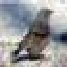
\includegraphics[]{figures/CIFAR10_example.pdf}};

\end{tikzpicture}




% % RECONSTRUCTION GRAPH
% \begin{tikzpicture}[node distance=1cm and 1.7cm, auto]
% %%Nodes

% \node (D) [minimum height=3.5cm] {\distribution};
% \node [above of= D, align=center, yshift=0.7cm] {data set \\ distribution};

% \node (A) [node, right= 1cm of D, fill=red!7, yshift=1.5cm] {\textbf{target} \\ $\set A$};
% \node (B) [node, right= 1cm of D, yshift=-1.5cm] {\textbf{original} \\ $\set B_\text{true}$}

% \node (Bp) [node, right= of B, fill=blue!3] {perturbed \\ \textbf{source} \\ $\set B$}; %\\ $\set B = \delta (\set B_\text{true})$};
% \node (Br) [node, right= of Bp, fill=blue!7] {\textbf{reconstructed} \\ $\rho (\set B)$};


% %%Arrows
% \draw [arrow, dashed, thin] (D) -- (A.190);
% \draw [arrow, dashed, thin] (D) -- (B.170);


% \draw [arrow, dashed, thin] (B) -- (Bp) 
% node (Pert) [midway, function, dashed] {$\delta$};
% \draw [linestart] (Bp) -- (Br) 
% node (Rec) [midway, function, draw=blue, fill=white] {$\rho$};
% \node [fill=white, below= 0cm of Rec] {\color{blue} \footnotesize optimize};
% \node [fill=white, below= 0cm of Pert] {\footnotesize \textit{unknown}};


% % \draw [dashed] (Rec) to [out=245, in=115] (Rec2);

% \node (Net) [function, thick, minimum width= 1cm, above right= -0cm and 3.1cm of A] {$\varphi$};
% \node [above right=-0.2cm and 0cm of Net] {\small feature-map};
% \node (Loss) [function, thick, above= 1.5cm of Net] {loss};

% \pgfmathtruncatemacro{\OutL}{110}
% \pgfmathtruncatemacro{\OutM}{95}
% \pgfmathtruncatemacro{\OutR}{75}
% \pgfmathtruncatemacro{\InL}{360-\OutL}
% \pgfmathtruncatemacro{\InM}{360-\OutM}
% \pgfmathtruncatemacro{\InR}{360-\OutR}

% \draw [lineend] (Net.\InL) to [corner connect h=-0.7cm] (A.east);
% \draw [arrowend] (Net.\OutL) to [out=90, in=270] (Loss.260);

% \draw [line] (Net.\InM) to [rect connect h=-0.7cm] (Br.100);
% \draw [arrowend] (Net.\OutM) to [out=90, in=270] (Loss.260);

% \draw [line, blue] (Net.\InR) to [rect connect h=-0.4cm] (Br.80);
% \draw [lineend, blue, connect v] (Net.\OutR) to (Loss.south);
% \draw [arrowend, blue, connect h] (Br.192) to (Rec.east);

% \path (Net.\OutL) -- node[midway, above= 0.15cm, sloped] {\small statistics}(Loss.260);
% % \node [above= 0.5cm of Net, fill=white] {\footnotesize optimize};
% % \draw [arrow, Mahogany, thin, bend left=20] (A) to node[near end, above] {\footnotesize trained} (Net);


% \end{tikzpicture}


    \caption{Outline of the Reconstruction task}
    \label{fig:outline}
    \centering
\end{figure}


We are given a data set $\set B$ 
and a neural network that was trained on - or performs reasonably well on - a data set $\set A$.
% The neural network is able to predict data coming from $\set A$ accurately, 
As the distribution of $\set B$ differs crucially from $\set A$, 
the neural network is unable to reach high performance on data coming from $\set B$.
The goal is to learn a transformation $\rho$ that adjusts $\set B$ 
so that the network's performance is regained.

An underlying assumption is that $\set B$ originates from the same distribution
as $\set A$, but has been corrupted by an unknown perturbation $\delta$.
The transformation $\rho$ is modeled to correct for this perturbation, 
in the sense that $\rho(\set B) \approx \set B_\text{true}$.
This is done by minimizing the a dissimilarity-score between $\set B$ and $\set A$ 
in a feature space given by an appropriate feature-map $\varphi$, 
after the transformation $\rho$ has been applied to $\set B$.
For this, simple statistics of both data sets, such as the mean and variance 
are recorded in feature space and $\rho$ is adjusted accordingly by backpropagation 
in order to make the statistics of the source $\set B$ approach those of the target $\set A$.

Whether matching statistics in feature space actually increases similarity between $\set A$ and $\set B$
strongly depends on $\varphi$ and its representation of the data set.

A hope is that the found transformation $\rho$ will be close to an inverse transformation
of $\delta$, i.e. that $\rho\circ\delta \approx \text{id}$, the identity transformation,
although it is important to note that this is different from saying that $\rho(\set B) \approx \set B_\text{true}$.


\subsection{Problem Formulation}
Given a feature-mapping $\varphi$, a source data set $\set B$ and a target data set $\set A$ - or simply the statistics of $\varphi(\set A)$,  find $\rho \in \mathcal{F}$, such that
\[
     \loss _\varphi (\set A, \rho(\set B)) \,,
\]
is minimized.
Here, the solution space $\mathcal F$ is a pre-defined set of functions, 
parametrized by $\boldsymbol \theta$.




%%%%%%%%%%%%%%%%%%%%%%%%%%%%%%%%%%%%%%%%%%%%%%%%
%%%%%%%%%%   Section: Inversion    %%%%%%%%%%%%%
%%%%%%%%%%%%%%%%%%%%%%%%%%%%%%%%%%%%%%%%%%%%%%%%


\section{Inversion}
\label{sec:Inversion}

\subsection{Objective outline}

\begin{figure}[h]
    \centering
    \begin{tikzpicture}[node distance=1.3cm and 1.4cm, auto]

%%Nodes
\node (D) [minimum height=3.5cm] {\distribution};
\node [above of= D, align=center, yshift=0.2cm] {data set \\ distribution};

\node (N) [below= -0.5cm of D, minimum height=3.5cm] {\noise};
\node [above of= N] {random noise};

\node (B) [node, right= of N, fill=blue!7, draw=blue, thick] {\textbf{Source} \\ $\set B$};
\node (A) [node, right= of D, fill=red!7] {\textbf{target} \\ $\set A$};

\path (A) -- (B) node (Mid) [midway] {};
\node (Net) [function, thick, minimum width=1cm, right= of Mid, xshift=1.2cm] {$\varphi$};
\node [below right= 0.1cm and -1.2cm of Net] {\small feature-map};
\node (Loss) [function, thick, right= of Net] {loss};

%%Arrows
% \pgfmathtruncatemacro{\InL}{160}
% \pgfmathtruncatemacro{\InM}{175}
% \pgfmathtruncatemacro{\InR}{195}
% \pgfmathtruncatemacro{\OutL}{360-\InL}
% \pgfmathtruncatemacro{\OutM}{360-\InM}
% \pgfmathtruncatemacro{\OutR}{360-\InR}
\pgfmathtruncatemacro{\OutL}{20}
\pgfmathtruncatemacro{\OutM}{5}
\pgfmathtruncatemacro{\OutR}{-15}
\pgfmathtruncatemacro{\InL}{180-\OutL}
\pgfmathtruncatemacro{\InM}{180-\OutM}
\pgfmathtruncatemacro{\InR}{180-\OutR}

\draw [arrow, dashed, thin] (D) -- (A);
\draw [arrow, dashed, thin] (N) -- (B);

\draw [linestart] (A.east) to [rect connect v=1cm] (Net.\InL);
\draw [arrowend] (Net.\OutL) to[out=0, in=180]  (Loss.170);

\draw [linestart] (B.15) to [rect connect v=1cm] (Net.\InM);
\draw [arrowend] (Net.\OutM) to[out=0, in=180] (Loss.170);

\draw [arrowend, blue] (Net.\InR) to[out=180, in=0, rect connect v=-0.5cm] (B.-5);
\draw [lineend, blue, connect h] (Net.\OutR) to (Loss.west);
\node [below= 0cm of B, yshift=-0cm] {\color{blue} \footnotesize optimize};

\path (Net) -- (Loss) node [above=0.3cm, midway] {\small statistics};
% \draw [arrow, Mahogany, thin, bend left=30] (A.20) to [out=40, in=140] node[above, sloped] {\footnotesize trained} (Net);

\node [below= 0cm of A] {\fbox{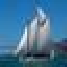
\includegraphics[]{figures/CIFAR10_example_3.pdf}}};

\end{tikzpicture}


    \caption{Outline of the Inversion task}
    \label{fig:inversion_outline}
    \centering
\end{figure}

A secondary part of this work is concerned about what kind of data 
may be recovered from having access to the statistics of a data set.
In this setting, we are given target statistics of data set $\set A$
and alternatively modify the source $\set B$ directly to 
minimize the dissimilarity just as outlined in \ref{sec:Reconstruction}.
The source data set is, in a first step, initialized randomly and then also 
iteratively refined by backpropagation after it has been mapped to feature-space.



\subsection{Problem Formulation}
Given a feature-mapping $\varphi$, the statistics of $\varphi(\set A)$
and target labels $\{y^{(i)}\}_{i=1}^{n_{\set B}}$ for a fixed integer size $n_{\set B}$,
find $\set B$, such that
\[
     \loss _\varphi (\set A, \set B)
\]
is minimized and $\set B = \{(\vec x^{(i)}, y^{(i)})\}_{i=1}^{n_{\set B}}$.

    


% \subsection{Problem Formulation}
% The result of the optimization process can be evaluated by calculating the accuracy obtained by $\Phi$. 
% Though, since $\Phi$ was used in the optimization process, it will likely display heavy bias to what it believes is a correctly classified sample.
% For this sake, another neural network $\Phi_{\text{ver}}$ can be employed, which has been separately trained on either $\set A$ or another data set. 

%Though, practice has shown that a very small portion of $\set A$ is only needed to obtain a close-enough guess at the true statistics of $\set A$.





\chapter{Experiments}
\label{chap:Experiments} 

The success of the reconstruction largely depends on the representation of the data
after the feature-map is applied.
Relying on the mean and variance of the data to accurately describe the data distribution 
relies on a strong assumption.
More sophisticated ways of capturing data distributions exist, yet mean and variance were chosen due to their simplicity in evaluation and computation of the gradients.

The feature-map ideally "disentangles" the data space to enable 
these simple statistics to capture enough of the complexity of the data set.

In order to assess the efficacy of the neural network's latent representations 
and their ability to capture the data distribution by these statistics,
several different mappings or methods will be compared. 

First, in order to establish the notation used throughout, in \cref{sec:nn_def}, 
a short introduction on the multi-layer perceptron (MLP) is given,
Then, the various feature-mappings or methods will be presented in \cref{sec:methods}.
Following that, the three data sets used in the experiments are introduced in \cref{sec:datasets},
and finally, the perturbation and reconstruction models are depicted in \cref{sec:reconstruction_models}.
\Cref{sec:evaluation} deals with evaluation metrics.

\section{Neural Network}
\label{sec:nn_def}

In a classification setting, a \textbf{neural network} $\Phi$ is a function that maps an input $\vec x \in \R^d$ to an output $\in \R^C$,
often referred to as the unnormalized logits. 
The network makes its prediction by returning the index of the maximal value of the logits.
The classic neural network is a \textbf{multi-layer perceptron} (MLP) or fully-connected (FC) neural network.
Here, every input of a layer is connected to every output of the layer.
Every node of any layer receives its input as a weighted sum over all of the previous layer's activations.
This weighted sum is passed through a non-linear activation function, often one of either the rectified-linear unit (ReLU) or sigmoid, to form the node's activation. 
This is done for all nodes in a layer before being passed on to the next.
A full network thus is a composition of functions $\Phi_\ell$, or \textbf{layers} that 
successively act on the outputs $\vec h$ of the previous layer, called \textbf{activations} or \textbf{hidden states}. 
In a plain \textbf{fully-connected} neural network, the layers are each made up of an affine linear transformation and a non-linear activation function.

Formally, a fully-connected neural network of layer depth L is described as:

\[
    \Phi : \R^d \to \R^C
\]
\[
    \Phi = \Phi_\text{L} \circ \ldots \circ \Phi_1
\]
\[
    \vec h_\ell = (\Phi_\ell \circ \ldots \circ \Phi_1) (\vec x) =
    \Phi_\ell(\vec h_{\ell-1}) \in \R^{d_\ell}
\]
$\Phi_\ell$ then, is a mapping from $\R^{d_{\ell-1}}$ to $\R^{d_\ell}$ and $\R^{d_\textnormal{L}} = \R^C$.
% The space of a hidden state $\vec h$ is called a \textbf{feature-space}.
The input $\vec x$ is sometimes also referred to as $\vec h_0$ and $\R^{d_0} := \R^d$.
The layers themselves contain as parameters a \textbf{weight matrix} $\vec W$ and a \textbf{bias} $\vec b$
that together form an affine linear transformation.
\[
    \Phi_\ell(\vec h) = \sigma (\vec W \vec h + \vec b) \comma{where}
    \vec W \in \R^{d_\ell \times d_{\ell-1}} \text{ and } 
    \vec b \in \R^{d_\ell}
\]

The non-linear activation function $\sigma$ is often a function $\sigma:\R\to\R$ that is applied element-wise.



\section{Methods}
\label{sec:methods}

The following methods introduce various feature-mappings.
Each feature-mapping $\varphi$ induces a loss function $\loss_\varphi$ as outlined in \cref{eqn:statistics_loss}.
For every method there exists a class-dependent loss formulation $\loss_\varphi^{\mathcal C}$,
as given in \cref{eqn:class_statistics_loss}.
The abbreviations to the methods are given in parenthesis in the following headers. 
When referring to the class-dependent formulation CC (class-conditional or
class-constrained) is added to the abbreviation.

The complete loss formulation that is used in the optimization process 
for a given feature-map $\varphi$, a target data set $\set A$ and a source data set $\set B$ 
is a composite loss given by
\[
    r_\text{stats}\loss_\varphi(\set A, \set B) + r_\text{crit}\loss_\text{crit}(\set B, y_{\set B}) \,,
\]
where $y_{\set B}$ are the target labels and $\loss_\text{crit}$ is the criterion loss, which, throughout this work, is the cross-entropy loss.
It is the loss function that was used for optimizing the parameters of the neural network.



\subsection{Neural Network - Second-to-Last Layer (NN)}

Given a neural network $\Phi$ of depth L,
a feature-mapping can be obtained by mapping inputs to the second-to-last layer $\Phi_{\text{L}-1}$, 
the layer before the logits layer.
\[
    \varphi : \R^d \to \R^{d_\textnormal{L-1}} = (\Phi_\textnormal{L-1} \circ \dots \circ \Phi_1)
\]
Generally, this layer is considered to encode a highly abstracted representation of the data
and typically contains the signal in a comparatively high dimensional space, before it's
reduction to a $C$-dimensional vector by the logits-layer.
% which contains the least amount of information  on the input.
In convolutional neural networks, where one often deals with images
of a specified input shape (the Cartesian product of channels$\times$height$\times$width), 
the spatial relationship of features is kept throughout the forward propagation by the layers.
In this layer, the entire signal is flattened down to a single $d^{\text{L}-1}$-dimensional vector, 
before being passed to the logits-layer.
As an activation function is normally not needed on the last layer when returning the index of the maximal value, 
the logits-layer has to be able to linearly classify its input - the last hidden state - in order to 
give the final prediction.
This warrants the belief that this layer contains the most disentangled representation of the data.


\subsection{Neural Network - All Layers (NN ALL)}

All hidden states together of the neural network can be seen as outputs of a collection of feature-maps [$\varphi_0, \dots, \varphi_\text{L}$], where
\begin{alignat*}{2}
    \varphi_\ell &: \R^d \to \R^{d_\ell} &&= (\Phi_\ell \circ \dots \Phi_1)
    \comma{for $\ell = 1, \dots$, L - 1}  \,, \\
    \varphi_\textnormal{L} &: \R^d \to \R^d &&= \Id \,.
\end{alignat*}





\subsection{Random Projections (RP)}
To contrast the efficacy of the previous two feature-representations on the success of the optimization process,
a feature-mapping involving one linear layer is used. This is done by selecting a number of  random linear projections.
A random projection is a linear mapping $r: \R^d \to \R$.
It is created by choosing a normalized random vector $\vec v \in S^{d-1} = \{\vec x \in \R^d : \|\vec x\| = 1\}$.
It can be seen as a linear projection to the one-dimensional subspace defined by the vector $\vec v \in \R^d$.
\[
    r(\vec x) = \vec v ^\top \vec x
\]
By choosing a total of $s_\text{RP}$ random vectors $\{v_1, \dots, v_{s_\text{RP}}\}$ one obtains a linear mapping $R: \R^d \to \R^n$:
\[
    R(\vec x) = \vec V \vec x =
    \begin{bmatrix}
        - \vec v_1 ^\top - \\
        \vdots \\
        - \vec v_n ^\top - \\
    \end{bmatrix}
    \vec x =
    \begin{bmatrix}
        \vec v_1 ^\top \vec x \\
        \vdots \\
        \vec v_n ^\top \vec x \\
    \end{bmatrix}
\]
%
% The loss function $\loss_R$ stays as was defined before.
In order to obtain a more balanced output,
the projection can be centered around an origin $\vec o$.
% 
\[
    R_{\vec o} (\vec x) = \vec V (\vec x - \vec o) \,,
\]
where $\vec o \in \R^d$ is the new origin of the projection. 
The idea is to set the origin to be center of the target data set $\set A$. $\vec o = \mean (\set A)$
This way, the data after the projection will be centered around $\vec 0$.
In practical applications, the data often is normalized and $\vec 0$-centered beforehand,
yet the class-dependent variant can be modified to select an origin $\vec o_c$ for each class $c$.
\cref{eqn:class_statistics_loss} then becomes:
% 
\begin{equation*}
    \loss _{\text{RP}} ^{\mathcal C} (\set A, \set B) =
    \sum _{c = 1, \dots, C}
    \begin{alignedat}[t]{1}
        \|\mean ({R_{\vec o_c} (\set A|_c)}) - \mean ({R_{\vec o_c} (\set B|_c)}) &\| \\
        {} + \|\var ({R_{\vec o_c} (\set A|_c)}) - \var ({R_{\vec o_c} (\set B|_c)}) &\|  \,,
    \end{alignedat}
\end{equation*}
% \begin{align}
% \begin{split}
% \label{eqn:class_statistics_loss}
%     \loss _\varphi ^\text{CC} (\set A, \set B) =
%     \sum _{c = 1, \dots, C}
%     \|\mean ({R_{\vec o_c} (\set A|_c)}) - \mean ({R_{\vec o_c} (\set B|_c)}) &\| \\
%     {} + \|\var ({R_{\vec o_c} (\set A|_c)}) - \var ({R_{\vec o_c} (\set B|_c)}) &\|  \,,
% \end{split}
% \end{align}
%
where $\vec o_c$ is set to the mean of each class $\mean ({\set A|_c})$.


\subsection{Random projections ReLU (RP ReLU)}
To further explore the importance of the non-linear activation functions contained within the network,
the previous method is modified by applying an activation function, in this case the ReLU to the output.
% 
\[
    R_{\vec o}^+ (\vec x) = (\vec V (\vec x - \vec o))^+ \,,
\]
where $(\,\cdot\,)^+ :\R^n \to \R^n$ is the projection onto the positive orthant. It applies $\max(0, \cdot)$ element-wise.

Since the layers of a neural network that use ReLU activation functions have a bias parameter that shifts the threshold above which an input can pass unaltered, this will also be incorporated.
\[
    R_{\vec o}^{\vec b} (\vec x) = (\vec V (\vec x - \vec o) + \vec b)^+ \,,
\]
where $\vec b \in \R^d$ is the bias. For a target dataset $\set A$, it is chosen as $\vec b \sim \mathcal N(\vec 0, \textnormal{diag}(\boldsymbol \sigma ^2))$, 
where $\boldsymbol \sigma ^2 = \var ({R_{\vec o}(\set A)})$.

The class-dependent variant can again make use of more suited biases $\vec b_c \sim \mathcal N( \vec 0, \textnormal{diag}(\boldsymbol \sigma _c^2))$, 
where $\boldsymbol \sigma_c ^2 = \var ({R_{\vec o_c}(\set A|_c)})$.
In this case, \cref{eqn:class_statistics_loss} becomes:
% 
\begin{equation*}
    \loss _{R^+} ^\text{CC} (\set A, \set B) =
    \sum _{c = 1 \dots C}
    \begin{alignedat}[t]{1}
        \|\mean ({R_{\vec o_c}^{\vec b_c} (\set A|_c)}) - \mean ({R_{\vec o_c}^{\vec b_c} (\set B|_c)}) &\| \\
        {} + \|\var ({R_{\vec o_c}^{\vec b_c} (\set A|_c)}) - \var ({R_{\vec o_c}^{\vec b_c} (\set B|_c)}) &\| 
    \end{alignedat}
\end{equation*}

\subsection{Randomly Initialized Neural Network (RANDOM NN)}
To further study the importance of an optimized feature-representation of a trained neural network, 
the same neural network model with randomly initialized parameters is evaluated and compared.
This could give insight to the importance of the number of compositions of non-linear transformations.

\subsection{Combinations (COMBINED)}
All previously defined feature-maps can be combined into a new collection of feature-maps,
in order to obtain a new loss formulation.
One combination in particular, the mixture of all neural network layers (NN ALL) and random projections (RP) is further examined in the following experiments.


\section{Data Sets}
\label{sec:datasets}

\subsection{GMM}
\label{sec:datasetgmm}
A dataset made up of Gaussian mixture models (in the following \textit{GMM}), 
is made up of $C$ classes, each of which contains $n_\text{mode}$ clusters or modes of multivariate Gaussian normal distributions. The probability-density function (pdf) is as follows.
\begin{align}
\label{eqn:gmm_distr}
    p(\vec x) &= \frac 1 C \sum_{c=1}^C p(\, \vec x \mid c \,) \nonumber\\
    p(\, \vec x \mid c \,) &= \frac 1 {n_\text{mode}} \sum _{m=1}^{n_\text{mode}}
    \mathcal N (\gamma \vec m_c + \lambda \boldsymbol \mu_c^{(m)}, \boldsymbol \Sigma_c^{(m)}) \, ,
\end{align}
where \\
$\vec m_c \sim \mathcal N (\vec 0, \vec I)$ is the center for each class $c=1,\ldots, C$ ,\\
$\boldsymbol \mu_c^{(m)} \sim \mathcal N (\vec 0, \vec I)$ and
$\vec \Sigma_c^{(m)}$ are the center and the covariance matrix of the multivariate normal distribution
for each mode $m=1,\ldots, n_{\textnormal{mode}}$ and class $c=1,\ldots, C$.  \\
A positive semi-definite matrix $\vec \Sigma_c^{(m)}$ is generated by choosing $d$ eigenvalues $\vec e = (e_1, \ldots, e_d)$, $e_i \sim \mathcal U(\alpha, \beta)$, for all $i=1, \ldots, d$, for some $\alpha, \beta > 0$ and 
by sampling a random orthogonal matrix $\vec Q$. 
This can be done for example by choosing $\vec Q = \{q_{ij}\}_{i,j=0}^{d}$, 
where $q_{ij} \sim \mathcal N(0, 1)$
and creating an orthonormal basis via Gram-Schmidt. 
\begin{align*}
    \vec \Sigma_c^{(m)} = \vec Q^\top \text{diag}(\vec e) \vec Q
\end{align*}

\begin{figure}[h]
    \centering
    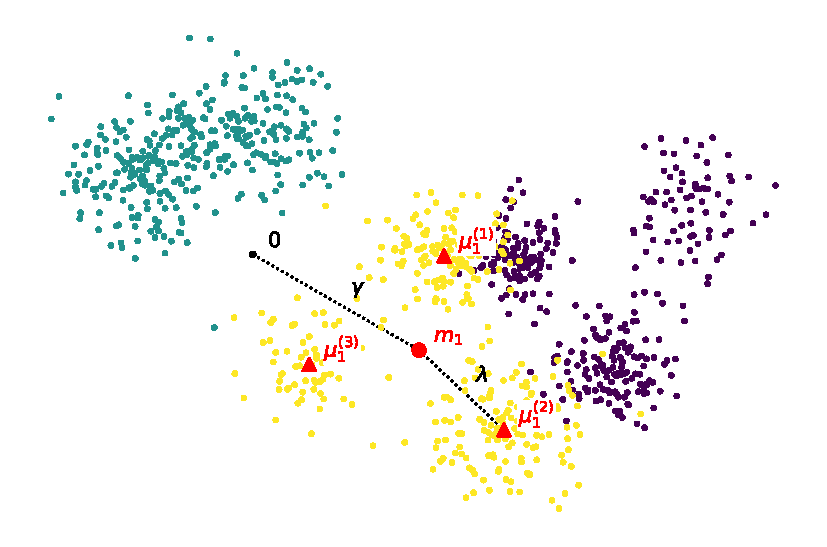
\includegraphics{figures/GMM_plot.pdf}
    \caption{GMM data set example for $d=2$, $C=3$, $n_\text{modes}=3$; 
    $\gamma$ and $\lambda$ control the standard-deviation of the distance of the class-center and the center of the modes respectively. $\alpha$ and $\beta$ control the size and orientation of the clusters}
    \label{fig:gmm_plot}
\end{figure}

For a given data set size, the labels are generated by equally sampling from all classes $1, \ldots, C$.
Then the input will be sampled according to the conditional probability-density function given by \cref{eqn:gmm_distr}.
The specific parameters used for generating the data set in all the experiments
are given in \cref{AppendixParameters}.


\subsection{MNIST}
MNIST, a common data set used in pattern recognition, is made up of 70000 black-and-white images 
of handwritten digits from 0 to 9. 
Each image is made up of 28$\times$28 pixels, totaling an input dimension of $d=784$.
\XXX{show example, give source}

\subsection{CIFAR-10}
CIFAR10 contains 60000 colored images from 10 non-overlapping categories or classes.
Each image has an input shape of $(3, 32, 32)$ as it comes with 3 color channels 
and has a dimension of 32$\times$32 pixels, resulting in a total of $d=3072$ dimensions.
\XXX{show example, give source}





\section{Perturbation and Reconstruction Models}
\label{sec:reconstruction_models}


\subsection{Gaussian Mixture Models}

The \textbf{perturbation} for the GMM data set is modeled by
a random affine-linear transformation.
The linear part consists of an identity transformation with added Gaussian noise
and the translation vector is also sampled by Gaussian noise.
The standard deviation of the noise is controlled by a parameter $\kappa > 0$.
\[
    \delta(\vec x) = (\vec I + \kappa \vec N)\vec x + \kappa \mu \,,
\]
where $\vec N = \{n_{i, j}\}_{i j = 1}^{d}$, $n_{ij} \sim \mathcal N (0, 1)$ for all $i, j = 1 , \ldots, d$
and 
$\mu = \{\mu_i\}_{i=0}^d$, $\mu_i \sim \mathcal N(0, 1)$ for all $i=1,\ldots,d$.
This transformation is in invertible if $\det (\vec I + \kappa \vec N) \neq 0$ with P=1,
\XXX{talk about invertibility?}
For $\kappa = 0$, the identity transformation is obtained.

The \textbf{reconstruction model} for this data set is also an affine-linear transformation. 
$\rho(\vec x) = \vec A \vec x + \vec b$.
$\vec A$ and $\vec b$ make up the model's learnable parameters, and
these are initialized to $\vec A = \vec I$ and $\vec b = \vec 0$ in order to form the identity transformation.
An optimal solution is given by
$\vec A^* = (\vec I + \kappa \vec N)^{-1}$, $\vec b^* = -\kappa \vec A^* \boldsymbol \mu$.
Proof:
\begin{equation}
\label{eqn:gmm_optimal}
\begin{split}
    \rho^* ( \delta (\vec x)) 
    &= \vec A^* ((\vec I + \kappa \vec N)\vec x + \kappa \boldsymbol \mu) + \vec b^* \\
    &= \vec A^* (\vec I + \kappa \vec N)\vec x + \kappa \vec A^* \boldsymbol \mu + \vec b^* \\
    &= \vec x
\end{split}
\end{equation}

\subsection{Image Data Sets}

\subsubsection{Perturbation Model}

The \textbf{perturbation model} for the image data sets MNIST and CIFAR10
is a composition of additive Gaussian noise and two noise-controlled 2d-convolutions.
\XXX{talk about 2d-convolutions?}

\[
    \delta(\vec x) = \vec K_2(\vec K_1(\vec x + \mu)
\]

The convolutions $\vec K_n$ are given by kernel matrices $\vec k_n$ of size $3\times3$ for $n=1,2$.
The kernel matrices are set to the identity kernel with added Gaussian noise, controlled by $\kappa$.
The identity kernel for the MNIST data set (which only contains one "color" channel) is given by 
% \eqnref{eqn:kernelid}.
\begin{equation*}
% \label{eqn:kernelid}
    \vec k_{\text{id}} = \begin{bmatrix}
        0 & 0 & 0 \\
        0 & 1 & 0 \\
        0 & 0 & 0 \\
    \end{bmatrix} \,.
\end{equation*}
For the CIFAR10 data set, where 3 color channels are present, the input shape is of (3, 32, 32). 
In order to obtain the same output shape, 
a total of $3*3=9$ convolution kernels $\vec k^{[i,j]}$ for $i,j=1,2,3$ are needed per convolution.
The output of channel $j$ is given by $\sum_{i=1}^{3} \vec x * \vec k^{[i, j]}$.
The identity convolution can be achieved by setting 
\[
    \vec k^{[i,j]} = \begin{cases}
        \vec k_{\text{id}} &, \text{ if } i = j\\
        \vec 0 &, \text{ otherwise} \\
    \end{cases} \,.
\]

This convolution operator is in general not invertible for $\kappa > 0$.
\XXX{Proof??}
Again, for $\kappa = 0$, the identity transformation is obtained.

For the output to contain the same dimensions as the input, the input needs to be \textit{padded}.
The 'reflection' padding was chosen.
\XXX{Should elaborate}


\subsubsection{Reconstruction Model}

\begin{figure}[!ht]
\begin{minipage}{0.5\textwidth}
\centering
\input{Figures/ChartInvertblock}
% \caption*{ResNet - Residual Layer}
\end{minipage}
\begin{minipage}{0.5\textwidth}
\centering
\begin{tikzpicture}[node distance=0.58cm and 1.7cm, auto]

\node [] (input) {Input};
\node [layer, below= 1cm of input, fill=Dandelion!9] (conv1) {Conv1x1};
\node [layer, below= of conv1] (res1) {Residual Layer};
\node [layer, below= of res1] (res2) {Residual Layer};
\node [below= of res2, minimum height=0.8cm] (res3) {\dots};
\node [layer, below= of res3] (res4) {Residual Layer};
% \node [layer, below= 1cm of input, fill=Dandelion!9] (conv1) {Conv3x3};
% \node [layer, below= of conv1, fill=Blue!5] (bn1) {BatchNorm};
% \node [layer, below= of bn1, fill=Mahogany!7] (relu) {ReLU};
% \node [layer, below= of relu, fill=Dandelion!9] (conv2) {Conv3x3};
% \node [layer, below= of conv2, fill=Blue!5] (bn2) {BatchNorm};
\node [below= 1cm of res4] (output) {Output};

% \path (input) -- node[anchor=center] (branch) {} (conv1);
% \path (bn2) -- node[circle, draw, minimum size=0.6cm, anchor=center] (plus) {} (output);
% \node at (plus) {+};

% \node [right= 1.6cm of branch] (dummy) {};
\node [draw, dashed, inner sep=0.25cm, fit=(res1)] {};

% \draw [larrow, rect connect v=2cm] (branch.center) to (plus.east);

\draw [larrow] (input) to (conv1);
\draw [larrow] (conv1) to (res1);
\draw [larrow] (res1) to (res2);
\draw [larrow] (res2) to (res3);
\draw [larrow] (res3) to (res4);
\draw [larrow] (res4) to (output);
% \draw [larrow] (bn1) to (relu);
% \draw [larrow] (relu) to (conv2);
% \draw [larrow] (conv2) to (bn2);
% \draw [larrow] (bn2) to (plus);
% \draw [larrow] (plus) to (output);


\end{tikzpicture}
% \caption*{ResNet - Residual Layer}
\end{minipage}
\caption{ResNet architecture}
\label{fig:resnet}
\XXX{add ReLU out + 1x1conv}
\end{figure}

The model for the reconstruction task on images is given by a residual network architecture
as outlined in \cref{fig:resnet}. 
The network \textit{width}, the number of individual convolutional kernels, is controlled by the parameter $s_\text{width}$; the \textit{depth}, the number of residual layers, by the parameter
$s_\text{depth}$.

The default parameters for the experiments are given in \cref{AppendixParameters}.




\section{Evaluation}
\label{sec:evaluation}

\begin{figure}[ht]
    \centering
    \begin{tikzpicture}[node distance=1cm and 1.7cm, auto]

\node (A) [node, fill=red!7] {\textbf{Target} \\ $\set A$};
\node (B) [node, below= of A] {\textbf{original} \\ $\set B_\text{true}$};
\node (C) [node, below= 2.2cm of B, fill=blue!0] {\textbf{Validation} \\ $\set C_{true}$};

\node (Bp) [node, right= of B, fill=blue!2] {perturbed \\ \textbf{Source} \\ $\set B$};
\node (Br) [node, right= of Bp, fill=blue!7] {\textbf{reconstructed} \\ $\rho^* (\set B)$};


\draw [arrow, dashed, thin] (B) -- (Bp) node (Pert) [midway, function, dashed] {$\delta$};
\draw [arrow] (Bp) -- (Br) node (Rec) [midway, function] {$\rho^*$};
\node [fill=white, below= 0cm of Pert] {\footnotesize \textit{unknown}};
\node [fill=white, below= 0cm of Rec] {\footnotesize \textit{learned}};


\node (Net) [function, fill=gray!5, above= of Br] {Neural \\ Network};
\node (vNet) [function, fill=gray!5, right= of Net] {verification \\ Neural \\ Network};

\draw [arrow, Mahogany, thin, bend left=20] (A) to (Net);
\draw [arrow, Mahogany, thin, bend left=20] (A) to node[below] {\footnotesize trained} (vNet);
\draw [arrow, Blue, thin] (Net.210) to[bend right=20] node [midway, above, sloped] {\footnotesize optimized} (Rec.north);

\node (Cp) [node, right= of C, fill=blue!0] {\textbf{perturbed} \\ $ {\set C}$};
\node (Cr) [node, right= of Cp, fill=blue!0] {\textbf{reconstructed} \\ $\rho ^*( {\set C})$};


\draw [arrow, dashed, thin] (C) -- (Cp);
\draw [arrow] (Cp) -- (Cr);

\draw [arrow, dashed, thin] (C) -- (Cp) node (Pert) [midway, function, dashed] {$\delta$};
\draw [arrow] (Cp) -- (Cr) node (Rec) [midway, function] {$\rho^*$};

\draw [arrow, <->, thin, OliveGreen] (Br.south) to [rect connect h=-0.75cm] (B.south);
\draw [arrow, <->, thin, OliveGreen] (Cr.north) to [rect connect h=0.75cm] (C.north);

\path (Br.east) to [out=0, in=270]  node [near end, OliveGreen, xshift=0.1cm] {accuracy} (vNet.265);
\draw [arrow, thin, OliveGreen] (Br.east) to [out=0, in=320] (Net.315);
\draw [arrow, thin, OliveGreen] (Cr.east) to [out=0, in=320] (Net.325);
\draw [arrow, thin, OliveGreen] (Cr.east) to [out=0, in=270] (vNet.south);


\node [OliveGreen] at ($(Bp)!0.5!(Cp)$) {IQA metrics};

\node [below= 1.5cm of Pert] (Id) {Id};
\path (Id) -| node[anchor=center] (Idr) {$\hat {\Id}$} (Rec);
\draw [arrow] (Id) -- 
node[near start, xshift=0.2cm, function] {$\delta$} 
node[near end, xshift=-0.2cm, function] {$\rho^*$} (Idr);
\draw [arrow, <->, thin, OliveGreen] (Idr.south) to [rect connect h=-0.6cm] (Id.south);
\node [OliveGreen, yshift=-1.2cm] at ($(Id)!0.5!(Idr)$) {rel. error};
% \node [circle, fill=blue] at (Idr){};
% \draw (0,0)|-node{mid}(2,3);
% \node [below= 1cm of Rec] {};
% \node (Cbelow) [below= of Cp] {EEE};
% \draw [arrow, dashed, thin] (C) -- (Cp) node (Pert) [midway, function, dashed] {$\delta$};
% \draw [arrow] (Cp) -- (Cr) node (Rec) [midway, function] {$\rho^*$};

\end{tikzpicture}
    \caption{Overview of evaluation metrics}
    \label{fig:evaluation_overview}
    \centering
\end{figure}

The result of the reconstruction task on the GMM data set can be evaluated by the \textbf{accuracy}
of the neural network. However, this however is likely to exhibit a strong bias in the classification accuracy 
towards the source data set $\set B$, as it, and 
the neural network 
are used in the optimization process
of many of the presented methods.
For this reason, the same transformations are applied to
a validation set $\set C$, and the 
correct classification rate will be reported as the \textbf{validation accuracy}. 
Because none of the data points in $\set C$
are used during optimization, it is, to some extent, a measure of generalization
of the learned transformation $\rho^*$.

A second measure of generalization can be made by evaluating the accuracy of an
independently trained neural network, the verification neural network.
The accuracy of the validation set $\set C$ on this second neural network 
constitutes the \textbf{verification accuracy}.

In the case of the GMM data set, since the explicit probability density function (pdf) is known, 
(see \ref{eqn:gmm_distr}), the estimated \textbf{cross-entropy}, given by
\begin{equation}
\label{eqn:cross_entropy}
    H(\set A) = - \frac 1 {|\set A|} \sum_{i=1}^{|\set A|} \log p(\vec x_i)
\end{equation}
is used as a measure of unlikelihood of $\set A$ coming from the underlying distribution.

% For the main reconstruction task, 
% five metrics will be studied to determine a methods success (along with visual appeal).
% For one, the accuracy of the reconstructed data set will be measured by the neural network.
% The relative l2-error, the peak signal-to-noise ratio, the accuracy of the neural network and the accuracy on a verification network.
% Alongside, a validation data set $\set C$ will measure generalization of the found reconstruction $\rho$ to a data set to which it was not optimized for.
% Since the original neural network was also used in the optimization process, a verification network $\Phi_{\text{ver}}$ will be used as a second evaluation of the accuracy.

If the perturbation $\delta$ is known, then one can calculate the \textbf{relative error} of the identity vectors. 
\begin{equation}
\label{eqn:fro_error}
    \varepsilon_F = \frac {\|\widehat {\vec I_d} - \vec I_d\|_F} {\|\vec I_d\|_F} \,,
\end{equation}
where $\widehat {\vec I_d} = \begin{pmatrix} \rho (\delta (\vec e_1), \dots, \rho (\delta (\vec e_d) \end{pmatrix}$ and $\vec e_i$ is the i-th unit vector of the standard basis.
%
Then \eqnref{eqn:fro_error} becomes
\begin{equation}
\label{eqn:l2_error}
    \varepsilon_F = \sqrt{ \frac 1 d \sum_{i=0}^d \|\rho (\delta (\vec e_i)) - \vec e_i)\|_2^2}
\end{equation}

Given an affine-transformation $\vec M \cdot + \vec s$,
% equation \ref{eqn:l2_error} becomes:

\begin{align*}
    &= \frac 1 d \sum_{i=1}^d \|\vec M \vec e_i + \vec s\|^2_2 \\
    &= \frac 1 d \sum_{i=1}^d \sum_{j=1}^d ( \vec M_{ij} + \vec s_j )^2 \\
    &= \frac 1 d \sum_{i=1}^d \sum_{j=1}^d \vec M_{ij}^2 + 2 \vec M_{ij} \vec s_j + \vec s_j^2 \\
    &= \frac 1 d \left (\| \vec M_{ij} \|_F^2 + d \| \vec s \|_2^2 + 2 \, \vec 1^\top \vec M \vec s \right )\\
    &\leq \| \vec M_{ij} \|_F^2 + \| \vec s \|_2^2 + 2 \|\vec 1^\top \vec M\|_2 \|\vec s\|_2\\
    &= \| \vec M_{ij} \|_F^2 + \| \vec s \|_2^2 + 2 \|\vec M\|_F \|\vec s\|_2\\
    &= \Bigl ( \| \vec M_{ij} \|_F + \| \vec s \|_2 \Bigr )^2
\end{align*}
Thus, for the GMM data set, where the distortion model $\delta(\vec x) = (\vec I + \kappa \vec N) \vec x + \kappa \boldsymbol \mu$
and reconstruction model $\rho(\vec x) = \vec A \vec x + \vec b$ are both 
affine-linear transformations, and the full transformation $\rho \circ \delta$ 
is expressed as $\vec A (\vec I + \kappa \vec N) \vec x + \kappa \vec A \boldsymbol \mu + \vec b$
this is motivated as follows.
\begin{align*}
    \varepsilon_F 
    &= \sqrt{ \sum_{i=1}^d \frac 1 d \|\rho(\delta (\vec e_i)) - \vec e_i \|_2^2 } \\
    &= \sqrt{ \sum_{i=1}^d \frac 1 d \left \| \Bigl ( \vec A (\vec I + \kappa \vec N) - \vec I \Bigr )\vec e_i 
        + (\vec b + \kappa \vec A \boldsymbol \mu ) \right \|_2^2} \\
    &\leq \| \vec A (\vec I + \kappa \vec N) - \vec I \|_F
        + \| \vec b + \kappa \vec A \boldsymbol \mu \|_2 \\
    &= \|(\vec A  - (\vec I + \kappa \vec N)^{-1})  (\vec I + \kappa \vec N)\|_F
        + \| \vec b + \kappa \vec A^* \boldsymbol \mu - \kappa \vec A^* \boldsymbol \mu + \kappa \vec A \boldsymbol \mu \|_2 \\
    &\leq \| \vec I + \kappa \vec N \|_F \|\vec A  - \vec A^* \|_F
        + \| \vec b - \vec b^*\|_2 + \| \kappa \vec A^* \boldsymbol \mu - \kappa \vec A \boldsymbol \mu \|_2 \\
    &\leq \| \vec I + \kappa \vec N \|_F \|\vec A  - \vec A^* \|_F
        + \| \vec b - \vec b^*\|_2 + \kappa \| \vec A^* - \vec A \|_F \\
    &= \left (\| \vec I + \kappa \vec N\|_F  + \kappa \right ) \|\vec A  - \vec A^* \|_F
        + \| \vec b - \vec b^*\|_2 \\
\end{align*}
where $\vec A ^*$ and $\vec b^*$ are the parameters to the exact inverse transformation of $\delta$ 
(see \ref{eqn:gmm_optimal}).
% For a unit vector $\vec e_i$ this becomes:
% \begin{equation*}
%     \|\rho(\delta (\vec e_i)) - \vec e_i \| 
%     \leq \|\vec I + \kappa \vec N\| \left(\|\vec A - \vec A^* \| 
%         + \|\vec b - \vec b ^*\| \right) \,.
% \end{equation*}
% \eqnref{eqn:fro_error} then, is bound by
% \begin{align*}
%     \varepsilon_F 
%     &\leq \|(\vec I + \kappa \vec N)\|
%     \sqrt{ \frac 1 d \sum_{i=0}^d \left(\|\vec A - \vec A^* \|  + \|(\vec b - \vec b ^*)  \| \right)^2} \\
%     &= \|(\vec I + \kappa \vec N)\| \left(\|\vec A - \vec A^* \|  + \|(\vec b - \vec b ^*)  \| \right) \,.
% \end{align*}

These calculations are no longer valid for the image data sets, as it is not guaranteed that 
an inverse transformation exists for the convolutional distortion models. The relative
error, as defined in \ref{eqn:l2_error} is reported, but it is important to
note that, due to the non-linear nature, the reconstruction model will behave differently 
for a unit-vector 
of the standard-basis than for an image from the data set.

A metric that is commonly encountered in image quality assessment (IQA), is the 
\textbf{peak signal-to-noise ratio} (\textbf{PSNR}).
It is formed between two images $\vec x$ and $\vec y$ and is calculated as follows.
\[
    PSNR(\vec x, \hat {\vec x}) = 20 \log_{10} \left (\frac {\max_i(\vec x_i)} {\|\vec x-\hat {\vec x}\|_2} \right )
\]
The PSNR is common measure of image quality when assessing image compression algorithms and is measured in decibels db.
It is similar to the relative error in that it uses the mean-squared error. 
However, it is assessed on data points directly and therefore could be more indicative of actual 
reconstruction quality, whereas the l2-error can be seen as a metric describing the 
overall distortion of the reconstruction.
For a batch of images, the score is averaged over the images to give an estimated mean PSNR score.

Both, the l2-error and the PSNR compare individual values in pixels of images for their calculations.
Because of this, a low score in both of these metrics might not necessarily mean that a reconstruction
model has a bad performance. A near optimal reconstruction function can suffer a heavy penalty
in these scores due to a slight shift in translation of pixel values that humans would not even be
able to notice.
These translations can easily occur in convolutional models.
For this reason, one last metric the, \textbf{structural similarity index measure} (\textbf{SSIM})
is considered. Since it does not compare individual pixel values, it is more robust to 
image translations.
It is given as follows.
\[
    \text{SSIM}(\vec x, \vec y) 
    = \frac {(2 \mu_{\vec x} \mu_{\vec y} + c_1)(2\sigma_{\vec x\vec y} + c_2)}
    {(\mu_{\vec x}^2 + \mu_{\vec y}^2 + c_1)(\sigma_{\vec x}^2 + \sigma_{\vec y}^2 + c_2)}
\]
\XXX{explain, talk rescale}



\section{Results}

\subsection{Quantitative Results}

\subsubsection{GMM}

All proposed methods are able to increase the main network's accuracy and validation accuracy.
Also, the accuracy of the verification network is increased.
It is interesting to note that even though nearly all methods decrease the 
the cross-entropy, the l2-error of the distortion always increases
- for a larger number of samples, the data set cross-entropy is reported as infinity.
This is due to floating point precision errors that arise even with overflow measures in place.
However, it is important to remember that the loss function used in the optimization process
is a composite loss from the proposed loss between the statistics
and the original cross-entropy loss used in the optimization of the neural network.
\[
    r_{stats} \loss(\set A, \set B) + r_{crit}\loss_{crit}(\set B, y_{\set B})
\]
Since, by itself, the original criterion loss alone already performs quite well, 
it can be said that the proposed losses act as a kind of regularization 
by incorporating more knowledge about the target data distribution that prevent overfitting
of the source data set.
A comparison of the results for the case $r_{crit}=0$ can be found in \cref{tab:gmm_results_raw}

The results shown in \cref{tab:gmm_results_raw} confirm the assumption that,
without any class information, no method is able to achieve good results.

In this scenario, two methods, namely NN CC and RP CC seem to give 
better generalization scores 
(validation and verification accuracy) than when the original cross-entropy loss 
$\loss_\text{crit}$ is included.
But it is hard to explain the lower cross-entropy when leaving out 
$\loss_\text{crit}$, which is specifically designed to minimize the cross-entropy.
Nevertheless it is important to note that scores can fluctuate a fair amount and more 
experiment runs are necessary to give a clearer picture.

\begin{table}[!htbp]
\centering
\footnotesize
\pgfplotstabletypeset[
results,
gmm,
display columns/0/.style={column name=\textbf{Baseline}, column type=l, string type},
]{figures/reconstruction_GMM_baseline.csv}
\caption{GMM baseline scores}
\label{tab:gmm_baseline}
\end{table}

\begin{table}[!htbp]
\centering
\footnotesize
\pgfplotstabletypeset[
results,
gmm,
every row 6 column 1/.style={highlight},
every row 8 column 1/.style={highlight},
every row 10 column 1/.style={highlight},
every row 11 column 1/.style={highlight},
every row 7 column 2/.style={highlight},
every row 4 column 3/.style={highlight},
every row 8 column 4/.style={highlight},
every row 8 column 5/.style={highlight},
]{figures/reconstruction_GMM_results.csv}
\caption{Metrics on reconstruction results after 100 optimization epochs on GMM data set}
\label{tab:gmm_results}
\end{table}

\begin{table}[!htbp]
\centering
\footnotesize
\pgfplotstabletypeset[
results,
gmm,
every row 1 column 1/.style={highlight},
every row 7 column 2/.style={highlight},
every row 7 column 3/.style={highlight},
every row 4 column 4/.style={highlight},
every row 7 column 5/.style={highlight},
]{figures/reconstruction_GMM_results_raw.csv}
\caption{Metrics on reconstruction results after 100 optimization epochs for $r_\text{crit}=0$ on GMM data set}
\label{tab:gmm_results_raw}
\end{table}


When reviewing the trajectories of the scores, many of the methods show that soon after
 the loss passes a reference value - the same loss calculated on a batch of 
unperturbed data - the l2-error is seen to increase. This can be seen in \cref{fig:metrics_GMM_l2_increase}.

\begin{figure}[!htbp]
    \centering
    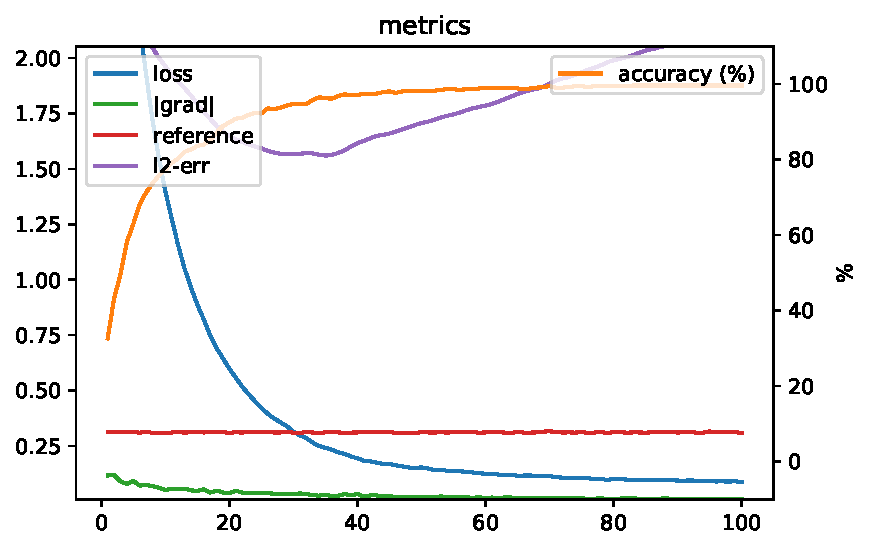
\includegraphics[width=0.7\textwidth]{figures/reconstruction_GMM_NN_ALL_metrics.pdf}
    \caption{Plot of optimization metrics of method NN ALL \\on the GMM data set}
    \label{fig:metrics_GMM_l2_increase}
\end{figure}

\subsubsection{MNIST}


The distortion factor ($\kappa = 0.2$) on the MNIST data set was chosen to be fairly strong.
After distortion, the overall accuracies drop from 97-99\% to near random guesses $\frac 1 C \approx 10\%$
as seen in \cref{tab:mnist_baseline}.
The results for the reconstruction task for all methods on the MNIST data set is depicted in \cref{tab:mnist_results}.
The criterion (CRITERION) alone gives leads to good results on the main network, but fails to generalize when tested on a secondary network.
This shows that the reconstruction is being heavily biased by what the neural network deems to be "correct" images, 
yet these features might not be robust in the sense that they don't correspond to features we as humans might make out.
The hardly improved verification score of NN, where additionally the second-to-last layer is 
incorporated, seems to confirm
the network's bias in the optimization procedure. 
An improvement in generalization can be seen only after taking 
all layers of the neural network (NN ALL) into account.
The randomly initialized neural network (RANDOM NN) does not add any significant improvement; 
it seems as though it is not able to capture much useful information about the data set.
Random projections (RP) is able to add an additional amount of regularization that is seen in the generalization scores.
Combining the methods (COMBINED) seems to merit overall good scores which can be verified in image quality.


\begin{table}[!htbp]
\centering
\footnotesize
\pgfplotstabletypeset[
results,
images,
display columns/0/.style={column name=\textbf{baseline}, column type=l, string type},
]{figures/reconstruction_MNIST_baseline.csv}
\caption{MNIST baseline scores}
\label{tab:mnist_baseline}
\end{table}

\begin{table}[!htbp]
\centering
\footnotesize
\pgfplotstabletypeset[
results,
images,
every row 11 column 1/.style={highlight},
every row 11 column 2/.style={highlight},
every row 11 column 3/.style={highlight},
every row 11 column 4/.style={highlight},
every row 5 column 5/.style={highlight},
every row 6 column 6/.style={highlight},
]{figures/reconstruction_MNIST_results.csv}
\caption{Metrics on reconstruction results after 100 optimization epochs on MNIST data set}
\label{tab:mnist_results}
\end{table}


Here, it is important to note that the l2-error and the PSNR-score do not improve after the reconstruction task is performed.
Comparing these findings with the qualitative results shown in \cref{AppendixResults}, 
leads to the conclusion that these scores are not actually indicative of image quality.
These scores rely on per-pixel comparisons, and the reconstruction network may introduce shifts in the final image
that can greatly disrupt the score of these metrics.
The SSIM-score seems to be a more robust metric, subjectively seen in image quality.





\subsubsection{CIFAR10}

The CIFAR10 data set is a more complex data set compared to the previous two.
The objects of interest have greatly varying backgrounds and are shown from numerous different angles.
The learned feature representations have to be able to filter out the noise from the signal more than in
the previous data sets.
The network for this data set is of a deeper (34 layers) architecture, and the
the learned feature representations seem to be more robust and correlate more with the verification network.
Comparing the results of the methods that use the representations of the main network (NN, NN ALL)
to the randomly initialized network (RANDOM NN), it can be said that a good feature representation is necessary.
Random projections do not perform well on this complex task, as their design is too simple.

\begin{table}[!htbp]
\label{tab:cifar10baseline}
\centering
\footnotesize
\pgfplotstabletypeset[
results,
images,
display columns/0/.style={column name=\textbf{Baseline}, column type=l, string type},
]{figures/reconstruction_CIFAR10_baseline.csv}
\caption{CIFAR10 baseline scores}
\end{table}

\begin{table}[!htbp]
\label{tab:cifar10results}
\centering
\footnotesize
\pgfplotstabletypeset[
results,
images,
every row 2 column 1/.style={highlight},
every row 4 column 1/.style={highlight},
every row 3 column 2/.style={highlight},
every row 4 column 3/.style={highlight},
every row 3 column 4/.style={highlight},
every row 3 column 5/.style={highlight},
every row 3 column 6/.style={highlight},
]{figures/reconstruction_CIFAR10_results.csv}
\caption{Metrics on reconstruction results after 100 optimization epochs for CIFAR10}
\end{table}





Of the methods using neural networks, NN ALL has the overall best performance.
This can be confirmed by visual inspection in \cref{AppendixResults}.
By using the class-conditional version (NN ALL CC), one would expect better results.
However, this is not seen in the results and the images appear qualitatively worse. 
A reason why could be that the network is already complex enough to "split" the signal into distinct enough paths so that adding
a class-conditional formulation does not add more context.
It might even be a hindrance, because of the high variance in image statistics
from one image to another due to background "noise".
Since the class-conditional formulation groups inputs according to their respective classes, 
it is possible that, due to random sampling, one iteration contains 
few samples of one class. Alternatively, one grouped batch could
display unusual statistics (e.g. all having red backgrounds).
This in turn can lead to a spike in the loss, resulting in large gradients that affect the optimization.
% NN ALL doesn't suffer from this, as irregularities are smoothed out by larger batches.
\Cref{fig:layer_losses} shows the loss resulting from the difference in the mean
between the source and the target, plotted for each layer.
While the normal formulation is able to minimize statistics over all layers relatively uniformly,
the class-conditional variation struggles with the early layers.
These exhibit higher losses that the reconstruction network is not able to minimize.
Solutions to this problem could entail an increase of the batch size
or, employing another batching method that randomly cycles over all classes
and then selects a batch accordingly. 
This could smooth out irregularities that arise from too few samples.
Alternatively, the losses could be weighted by their layer, giving lower importance to earlier layers. 
Or a hybrid approach could be constructed that only uses class information in later layers.

\begin{figure}
    \centerline{
    \hspace*{6mm}
    \begin{minipage}{0.6\textwidth}
    \caption*{NN ALL}
    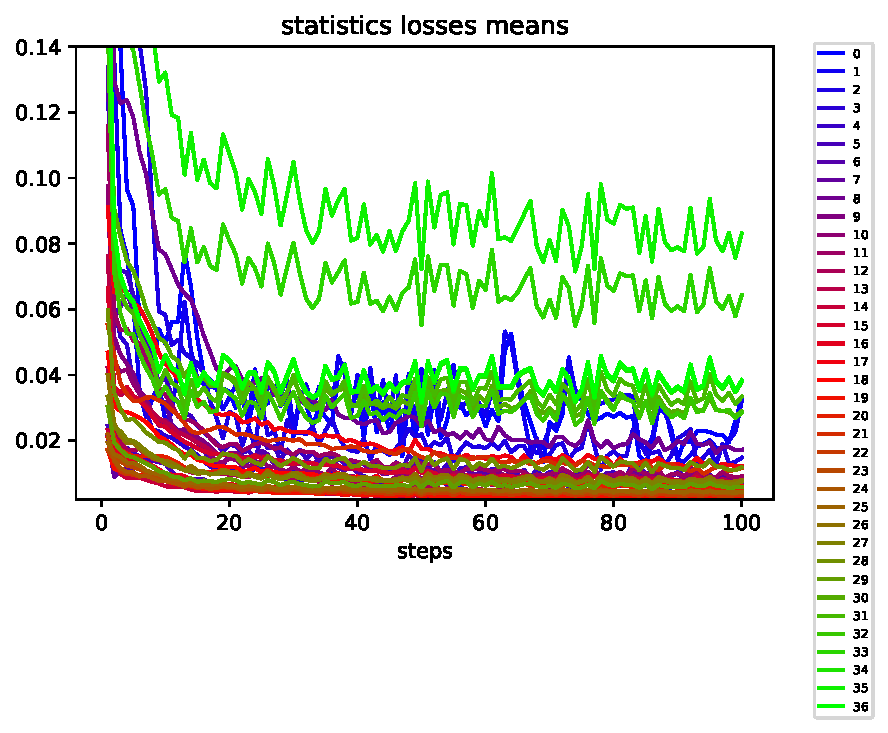
\includegraphics[
    width=\textwidth, 
    trim={0 0 0 0.6cm}, clip,
    ]{figures/reconstruction_CIFAR10_NN_ALL_metrics_statistics_losses_means.pdf}
    \end{minipage}%
    \begin{minipage}{0.6\textwidth}
    \caption*{NN ALL CC}
    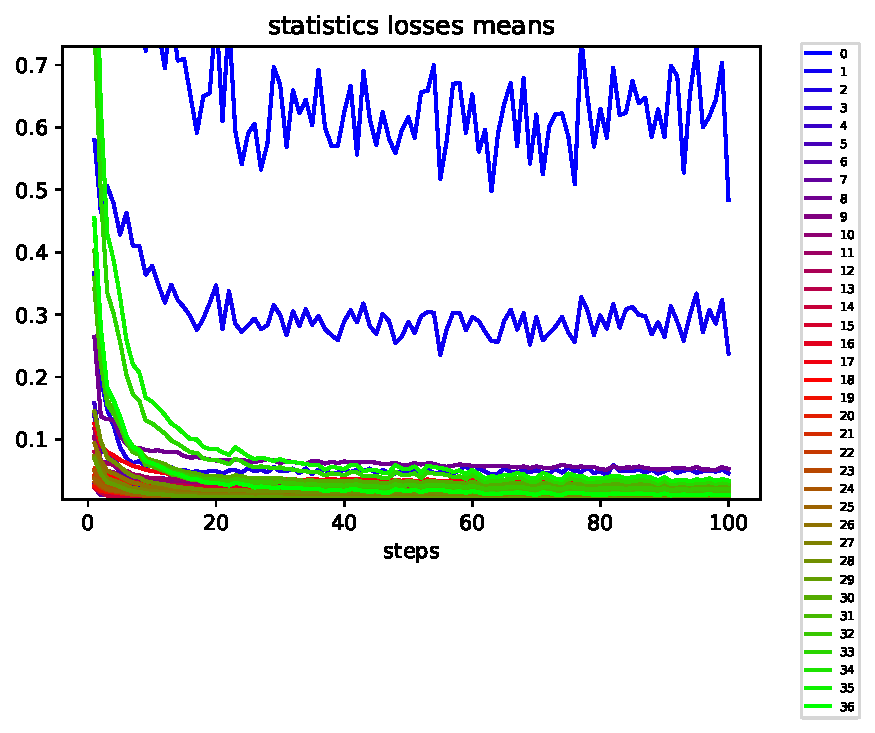
\includegraphics[
    width=\textwidth,
    trim={0 0 0 0.6cm}, clip,
    ]{figures/reconstruction_CIFAR10_NN_ALL_CC_metrics_statistics_losses_means.pdf}
    \end{minipage}
    }
    \caption{Loss coming from the difference in mean batch-statistics plotted per layer. 
    Lighter colors correspond to later layers in the network. \textit{Layer 0} is the input itself.}
    \label{fig:layer_losses}
\end{figure}



Conclusion:...
Incorporating the non-linearity ReLU in the random projections (RP ReLU), in general, 
does not seem to lead to any notable differences of the performance.



\subsection{Hyperparameter-Influence}


In the following, the influence of various hyperparameter settings on the reconstruction outcome is studied.
A grid search is performed on:
\begin{flalign*}
    s_\text{width} &\in \{4, 8, 16\} &\\
    s_\text{depth} &\in \{4, 8, 16\} \\
    n_{\set B} &\in \{128, 512, 1024, 2048\} \\
\end{flalign*}

Every run depicts a hyperparameter setting ($s_\text{width}, s_\text{depth},  n_{\set B}$) of the Cartesian product
of all possible values shown above.

The results for the reconstruction task are plotted in \cref{fig:rec_hyperparameter_search}.

The influence of $n_{\set B}$ on the outcome is quite clear, but the width and the depth of the reconstruction
network is not. In fact, it might even seem as though an increase in complexity of the model is rather
detrimental to the scores.

The findings are solidified in \cref{fig:rec_hyperparameter_heatmap}, where a correlation heat map is given
between the parameters and the scores is given.

While $n_{\set B}$ is clearly positively correlated for all scores 
(except for the l2-error, where a lower score is better), 
the other parameters show an almost inverse effect on what one would expect.
The larger reconstruction models would likely achieve higher scores after a longer training time.






\begin{figure}[!htbp]
\centering
    
    \caption*{\hspace*{6mm}NN ALL CC}
    \centerline{
    \hspace*{6mm}
    \begin{minipage}{0.6\textwidth}
    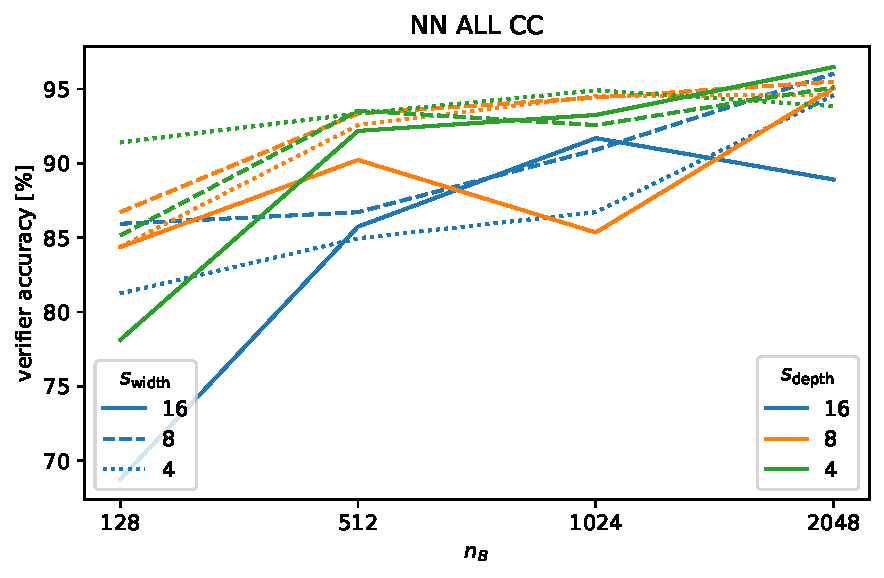
\includegraphics[
    trim={0 0 0 0.6cm}, clip,
    width=\textwidth
    ]{figures/comparison_CIFAR10_hyperparameters_verifier_accuracy_NN_ALL_CC.pdf}
    \end{minipage}%
    \begin{minipage}{0.6\textwidth}
    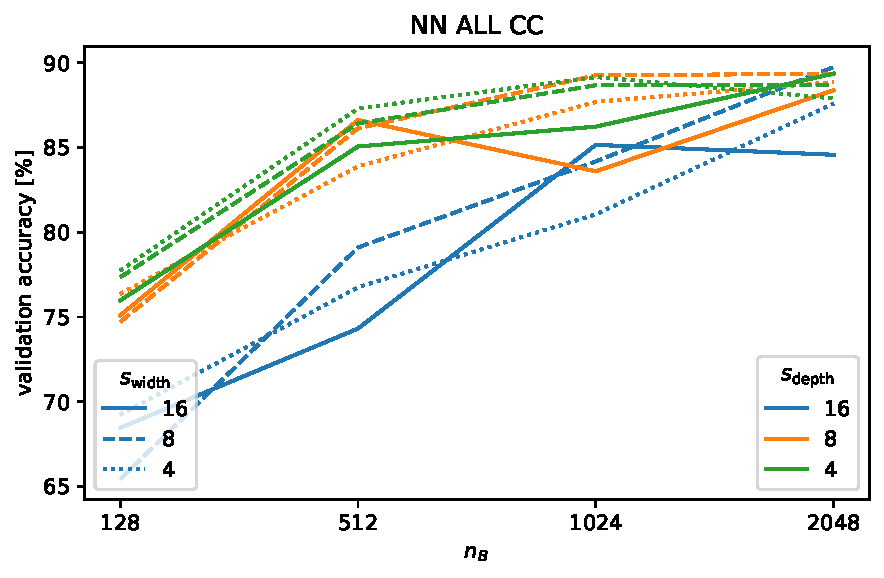
\includegraphics[
    trim={0 0 0 0.6cm}, clip,
    width=\textwidth
    ]{figures/comparison_CIFAR10_hyperparameters_validation_accuracy_NN_ALL_CC.pdf}
    \end{minipage}
    }
\caption{Reconstruction Results for multiple hyperparameter settings on CIFAR10. 
Every data point depicts the end-results after 100 epochs.}
\label{fig:rec_hyperparameter_search}
\end{figure}


\begin{figure}[!htbp]
\centering
\caption*{NN ALL CC}
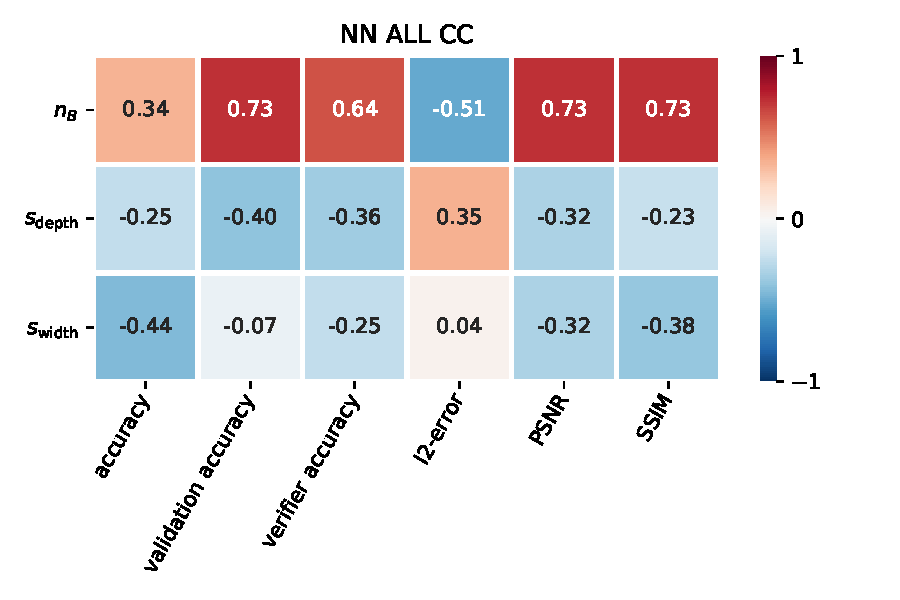
\includegraphics[
trim={0 0 0 0.75cm}, clip,
width=0.7\textwidth
]{figures/comparison_CIFAR10_hyperparameters_heatmap_NN_ALL_CC.pdf}
\caption{hyperparameter correlation table}
\label{fig:rec_hyperparameter_heatmap}
\end{figure}






















\appendix % Cue to tell LaTeX that the following "chapters" are Appendices
\chapter{Implementation Details}
\label{AppendixGlossary}


The implementation of this work was done in Python\footnote{\url{https://www.python.org/}}
using the popular machine-learning library PyTorch\footnote{\url{https://pytorch.org/}}.
A copy of the code repository along with all the results 
is made publicly available on Github\footnote{\url{https://github.com/willisk/Thesis}}.

\begin{table}[!h]
\caption*{\Large\textbf{Glossary}\vspace{1cm}}
\pgfplotstabletypeset[
glossary,
every row no 5/.style={extra spacing},
]{
scalar & $s$ & small letters are used for scalars
vector & $\vec v$ & bold-face small letters are used for vectors,
&& the elements are denoted as $v_i$
matrix & $\vec M$ & bold-face capital letters are used for matrices,
&& the elements are denoted as $M_{i,j}$
identity matrix & $\vec I$ & denotes the identity matrix
%
sample input & $\vec x$ & element of input space $\set X$
input space & $\set X$ & vector space $\R^d$
data set dimension & $d$ & dimension of vector space $\set X$
input shape & $(d_1, d_2,\ldots)$ & shape of input sample $\vec x \in \R^d=\R^{d_1\times d_2 \times \ldots}$
sample label & $y$ & label $y \in \set Y$
label set &$\set Y$ & discreet set $\set Y = \{1,\ldots, C\}$
number of classes &$C$ & number of distinct labels/classes of the data set
sample & $\vec z$ & sample of $\set Z$; tuple of input and label $\vec z = (\vec x, y)$
sample space & $\set Z$ & $\set Z = \set X \times \set Y$
%
& $\finiteset{\, \cdot \,}$ & denotes the set of all finite non-empty subsets
target data set & $\set A$ & data set $\set A = \{\vec z^{(i)}\}_{i=1}^{|\set A|}$ containing samples of $\set Z$;
&&used for training the main network, 
&&and for target data set statistics
source data set & $\set B$ & used in optimization,
&&where source data set statistics are to 
&&match target data set statistics
validation data set & $\set C$ & used for evaluating validation accuracy
class-constrained batch & $\set A|_c$ & subset of $\set A$ only containing samples of label c 
%(as defined in \ref{eqn:class_constrained})
input mean & $\mean$ & empirical data set sample input mean (defined in \ref{eqn:sample_mean})
input variance & $\var$ & empirical data set sample input variance (defined in \ref{eqn:sample_var})
feature-mapping & $\varphi(\set A)$ & maps a data set to feature-space (defined in \ref{eqn:feature_mapping})
statistics-loss & $\loss_\varphi$ & loss/objective function for given feature-mapping $\varphi$ 
&&(defined in \ref{eqn:statistics_loss})
class-loss & $\lossCC_\varphi$ & class-dependent formulation of loss function (defined in \ref{eqn:class_statistics_loss})
normal distribution & $\mathcal N (\boldsymbol \mu, \boldsymbol \Sigma)$ & multivariate normal distribution 
&&with mean $\boldsymbol \mu$ and covariance-matrix $\boldsymbol \Sigma$
uniform distribution & $\mathcal U (a, b)$ & continuous uniform distribution over interval $(a, b)$
}
\end{table}

\chapter{Results}
\label{AppendixResults}



\begin{figure}
    \centerline{
    \hspace*{6mm}
    \begin{minipage}{0.6\textwidth}
    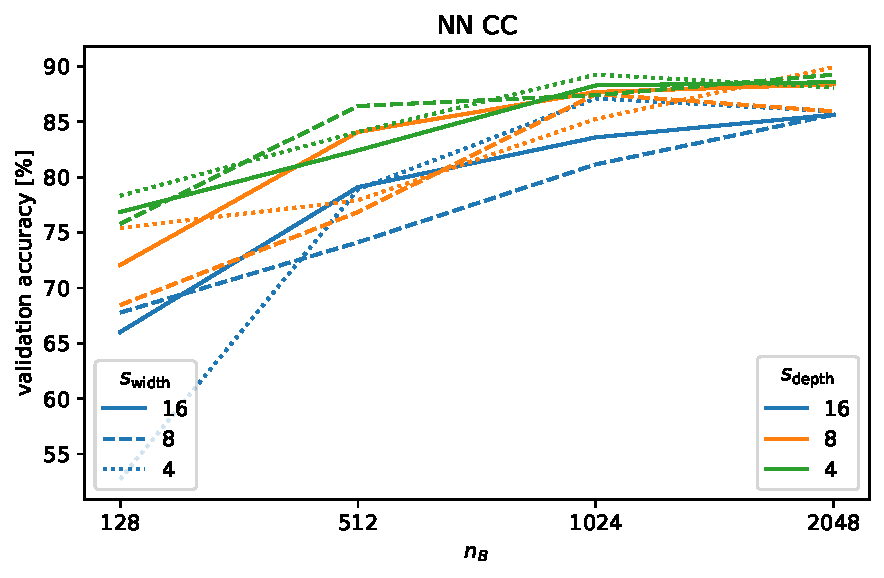
\includegraphics[width=\textwidth]{figures/comparison_CIFAR10_hyperparameters_validation_accuracy_NN_CC.pdf}
    \end{minipage}%
    \begin{minipage}{0.6\textwidth}
    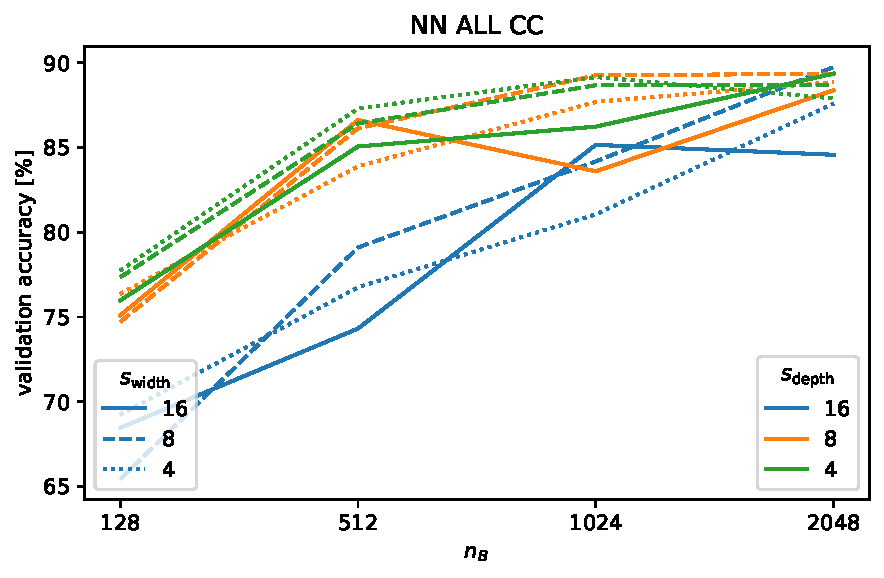
\includegraphics[width=\textwidth]{figures/comparison_CIFAR10_hyperparameters_validation_accuracy_NN_ALL_CC.pdf}
    \end{minipage}
    }
    \centerline{
    \hspace*{6mm}
    \begin{minipage}{0.6\textwidth}
    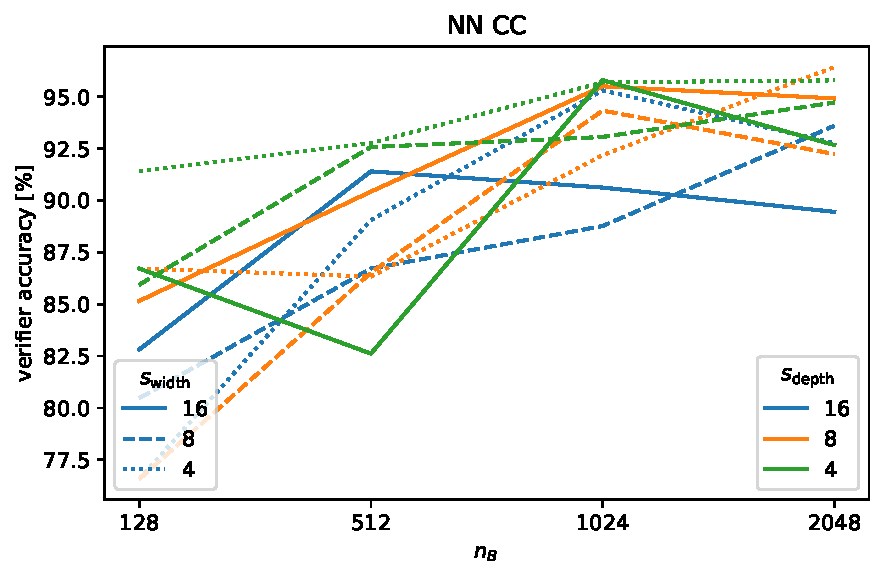
\includegraphics[width=\textwidth]{figures/comparison_CIFAR10_hyperparameters_verifier_accuracy_NN_CC.pdf}
    \end{minipage}%
    \begin{minipage}{0.6\textwidth}
    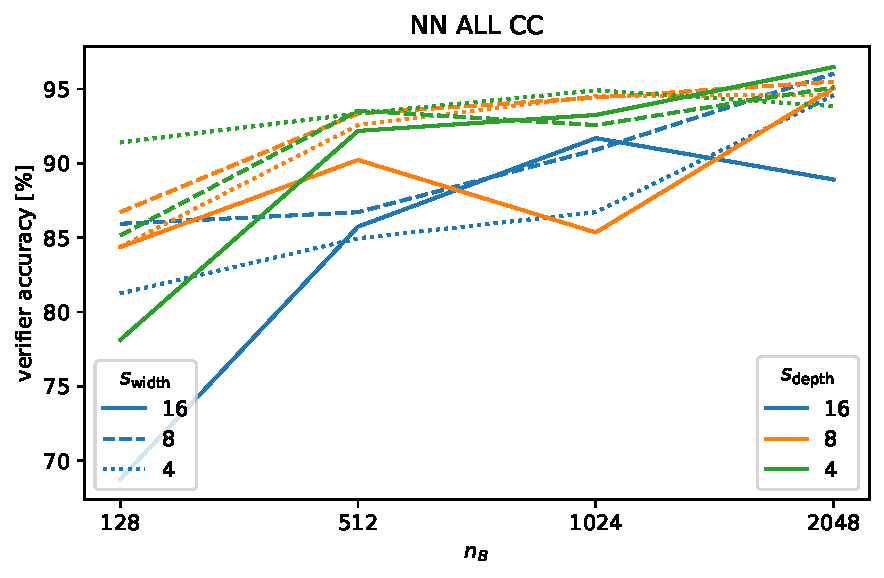
\includegraphics[width=\textwidth]{figures/comparison_CIFAR10_hyperparameters_verifier_accuracy_NN_ALL_CC.pdf}
    \end{minipage}
    }
    \centerline{
    \hspace*{6mm}
    \begin{minipage}{0.6\textwidth}
    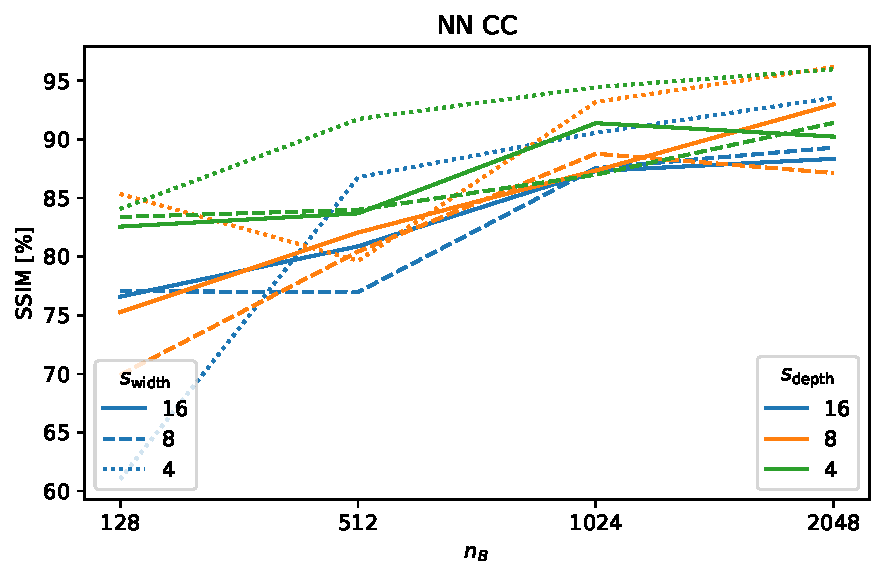
\includegraphics[width=\textwidth]{figures/comparison_CIFAR10_hyperparameters_SSIM_NN_CC.pdf}
    \end{minipage}%
    \begin{minipage}{0.6\textwidth}
    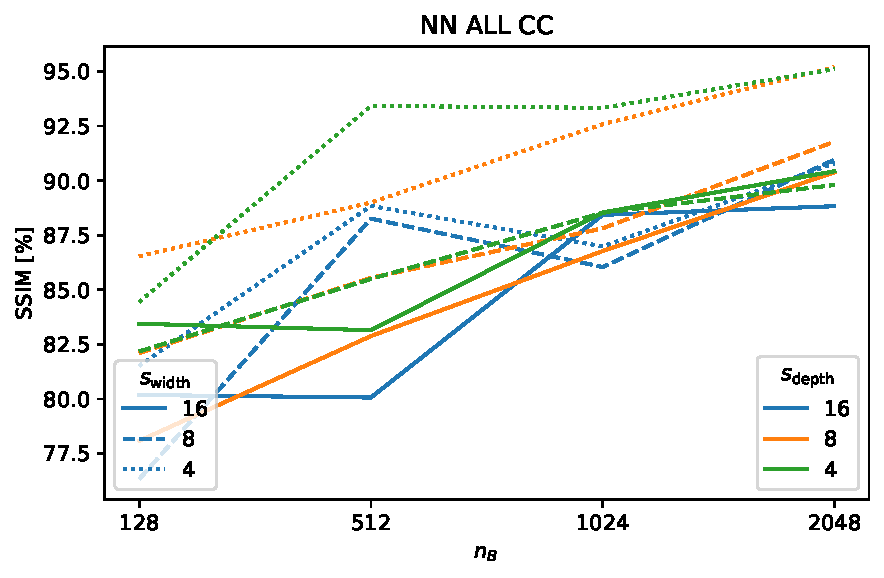
\includegraphics[width=\textwidth]{figures/comparison_CIFAR10_hyperparameters_SSIM_NN_ALL_CC.pdf}
    \end{minipage}
    }
    \caption{Hyperparameter influence on metrics}
    % \centerline{
    % \hspace*{6mm}
    % \begin{minipage}{0.6\textwidth}
    % 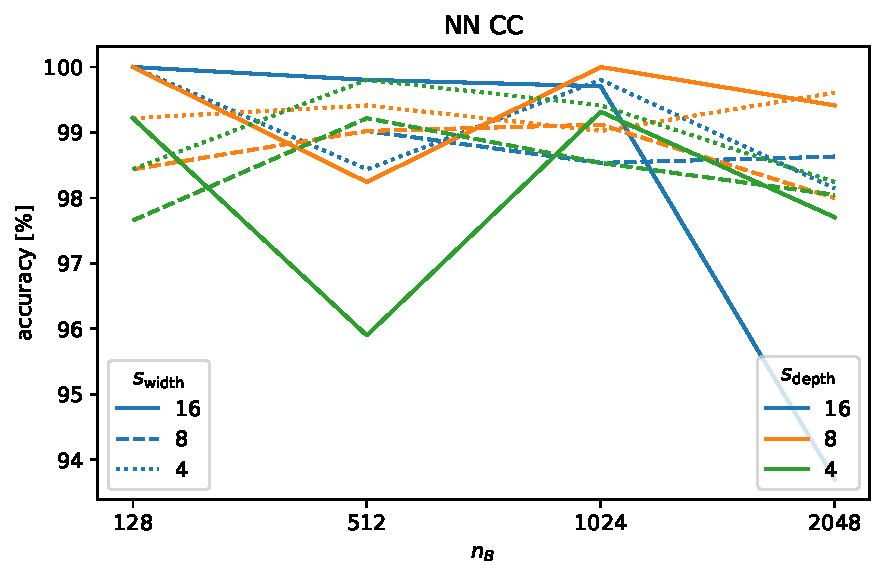
\includegraphics[width=\textwidth]{figures/comparison_CIFAR10_hyperparameters_accuracy_NN_CC.pdf}
    % \end{minipage}%
    % \begin{minipage}{0.6\textwidth}
    % 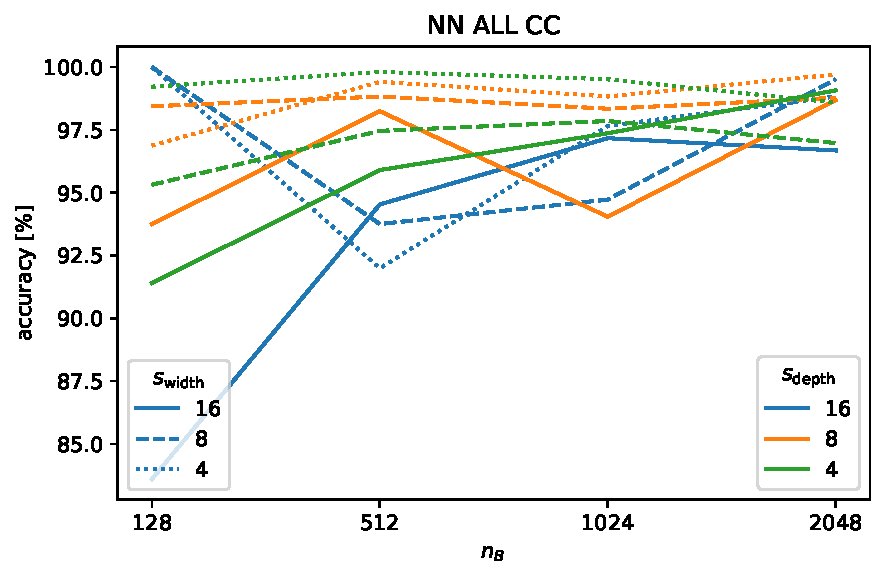
\includegraphics[width=\textwidth]{figures/comparison_CIFAR10_hyperparameters_accuracy_NN_ALL_CC.pdf}
    % \end{minipage}
    % }
    \label{fig:HyperparamInfluence}
\end{figure}



\begin{figure}
    \centering
    \setlength{\abovecaptionskip}{0pt plus 0pt minus 0pt}
    \setlength{\belowcaptionskip}{16pt plus 0pt minus 0pt}
    
    \caption*{\normalsize{\textit{Ground Truth}}}
    \rule{0.4\textwidth}{.4pt}
    
    \centerline{\hspace*{8mm}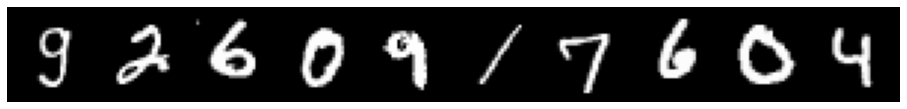
\includegraphics[width=1.4\textwidth]{figures/reconstruction_MNIST_ground_truth.png}}
    \caption*{\normalsize{\textit{Distorted}}}
    \rule{0.4\textwidth}{.4pt}
    
    \centerline{\hspace*{8mm}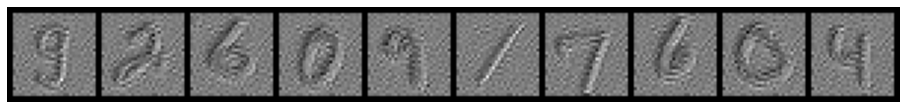
\includegraphics[width=1.4\textwidth]{figures/reconstruction_MNIST_distorted.png}}
    \caption*{\normalsize{CRITERION}}
    \rule{0.4\textwidth}{.4pt}
    
    \centerline{\hspace*{8mm}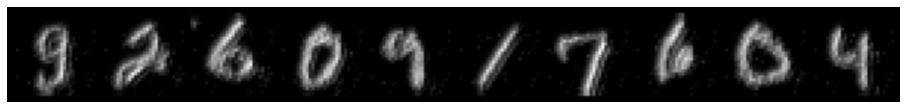
\includegraphics[width=1.4\textwidth]{figures/reconstruction_MNIST_CRITERION_epoch_100.png}}
    \caption*{\normalsize{NN}}
    \rule{0.4\textwidth}{.4pt}
    
    \centerline{\hspace*{8mm}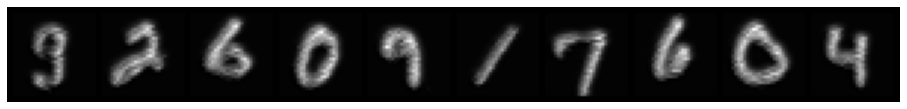
\includegraphics[width=1.4\textwidth]{figures/reconstruction_MNIST_NN_epoch_100.png}}
    \caption*{\normalsize{NN CC}}
    \rule{0.4\textwidth}{.4pt}
    
    \centerline{\hspace*{8mm}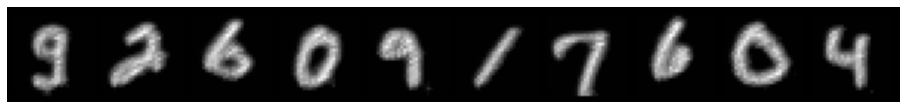
\includegraphics[width=1.4\textwidth]{figures/reconstruction_MNIST_NN_CC_epoch_100.png}}
    \caption*{\normalsize{NN ALL}}
    \rule{0.4\textwidth}{.4pt}
    
    \centerline{\hspace*{8mm}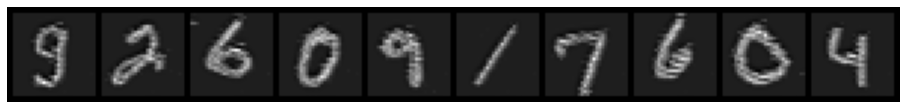
\includegraphics[width=1.4\textwidth]{figures/reconstruction_MNIST_NN_ALL_epoch_100.png}}
    \caption*{\normalsize{NN ALL CC}}
    \rule{0.4\textwidth}{.4pt}
    
    \centerline{\hspace*{8mm}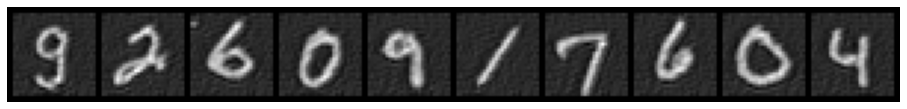
\includegraphics[width=1.4\textwidth]{figures/reconstruction_MNIST_NN_ALL_CC_epoch_100.png}}
    \label{fig:MNIST_Images}
\end{figure}
\begin{figure}
    \centering
    \setlength{\abovecaptionskip}{0pt plus 0pt minus 0pt}
    \setlength{\belowcaptionskip}{16pt plus 0pt minus 0pt}
    \caption*{\normalsize{RANDOM NN}}
    \rule{0.4\textwidth}{.4pt}
    
    \centerline{\hspace*{8mm}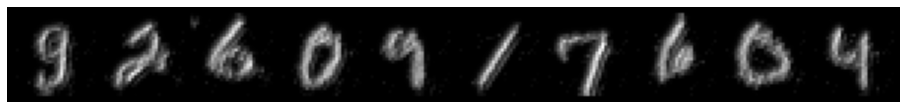
\includegraphics[width=1.4\textwidth]{figures/reconstruction_MNIST_RANDOM_NN_epoch_100.png}}
    \caption*{\normalsize{RANDOM NN CC}}
    \rule{0.4\textwidth}{.4pt}
    
    \centerline{\hspace*{8mm}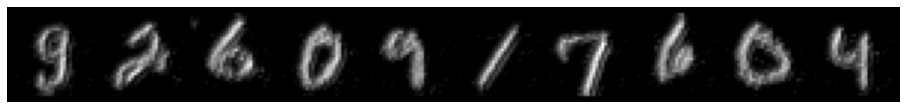
\includegraphics[width=1.4\textwidth]{figures/reconstruction_MNIST_RANDOM_NN_CC_epoch_100.png}}
    \caption*{\normalsize{RP}}
    \rule{0.4\textwidth}{.4pt}
    
    \centerline{\hspace*{8mm}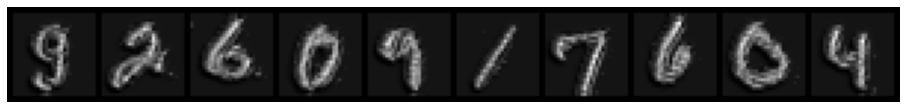
\includegraphics[width=1.4\textwidth]{figures/reconstruction_MNIST_RP_epoch_100.png}}
    \caption*{\normalsize{RP CC}}
    \rule{0.4\textwidth}{.4pt}
    
    \centerline{\hspace*{8mm}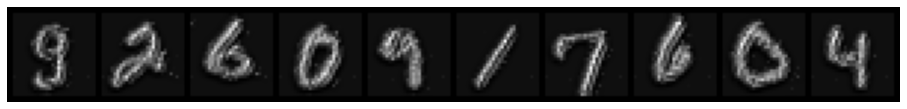
\includegraphics[width=1.4\textwidth]{figures/reconstruction_MNIST_RP_CC_epoch_100.png}}
    \caption*{\normalsize{RP ReLU}}
    \rule{0.4\textwidth}{.4pt}
    
    \centerline{\hspace*{8mm}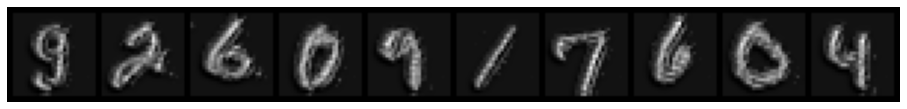
\includegraphics[width=1.4\textwidth]{figures/reconstruction_MNIST_RP_ReLU_epoch_100.png}}
    \caption*{\normalsize{RP ReLU CC}}
    \rule{0.4\textwidth}{.4pt}
    
    \centerline{\hspace*{8mm}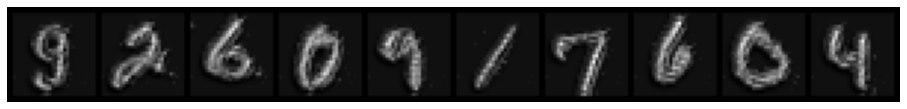
\includegraphics[width=1.4\textwidth]{figures/reconstruction_MNIST_RP_ReLU_CC_epoch_100.png}}
    \caption*{\normalsize{COMBINED CC}}
    \rule{0.4\textwidth}{.4pt}
    
    \centerline{\hspace*{8mm}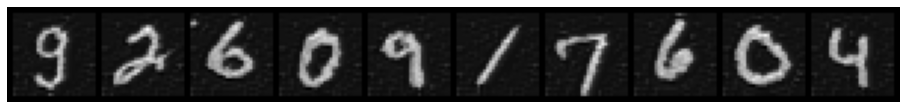
\includegraphics[width=1.4\textwidth]{figures/reconstruction_MNIST_COMBINED_CC_epoch_100.png}}
\end{figure}




\begin{figure}
    \centering
    \setlength{\abovecaptionskip}{0pt plus 0pt minus 0pt}
    \setlength{\belowcaptionskip}{16pt plus 0pt minus 0pt}
    \caption*{\normalsize{\textit{Ground Truth}}}
    \rule{0.4\textwidth}{.4pt}
    
    \centerline{\hspace*{8mm}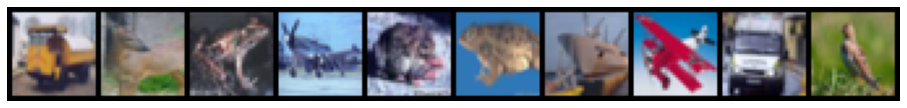
\includegraphics[width=1.4\textwidth]{figures/reconstruction_CIFAR10_ground_truth.png}}
    \caption*{\normalsize{\textit{Distorted}}}
    \rule{0.4\textwidth}{.4pt}
    
    \centerline{\hspace*{8mm}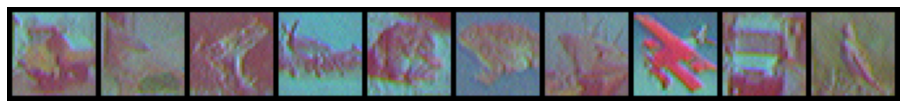
\includegraphics[width=1.4\textwidth]{figures/reconstruction_CIFAR10_distorted.png}}
    \caption*{\normalsize{CRITERION}}
    \rule{0.4\textwidth}{.4pt}
    
    \centerline{\hspace*{8mm}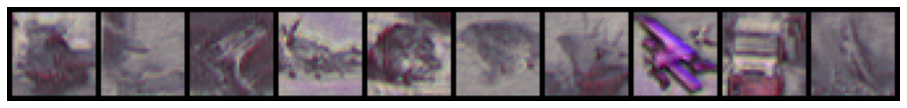
\includegraphics[width=1.4\textwidth]{figures/reconstruction_CIFAR10_CRITERION_epoch_100.png}}
    \caption*{\normalsize{NN}}
    \rule{0.4\textwidth}{.4pt}
    
    \centerline{\hspace*{8mm}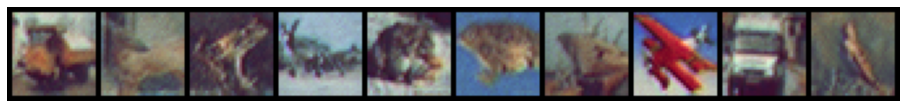
\includegraphics[width=1.4\textwidth]{figures/reconstruction_CIFAR10_NN_epoch_100.png}}
    \caption*{\normalsize{NN CC}}
    \rule{0.4\textwidth}{.4pt}
    
    \centerline{\hspace*{8mm}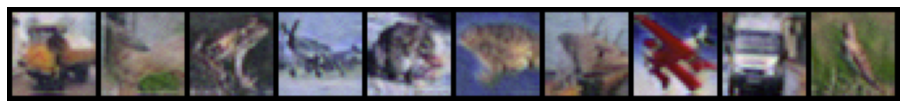
\includegraphics[width=1.4\textwidth]{figures/reconstruction_CIFAR10_NN_CC_epoch_100.png}}
    \caption*{\normalsize{NN ALL}}
    \rule{0.4\textwidth}{.4pt}
    
    \centerline{\hspace*{8mm}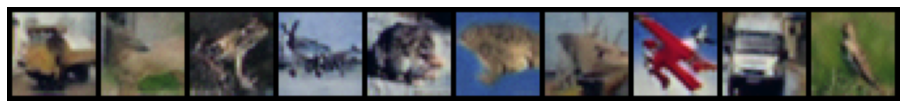
\includegraphics[width=1.4\textwidth]{figures/reconstruction_CIFAR10_NN_ALL_epoch_100.png}}
    \caption*{\normalsize{NN ALL CC}}
    \rule{0.4\textwidth}{.4pt}
    
    \centerline{\hspace*{8mm}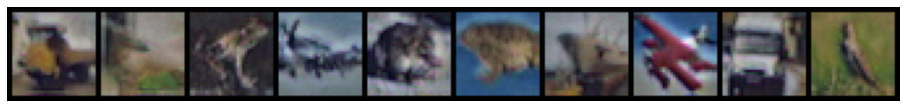
\includegraphics[width=1.4\textwidth]{figures/reconstruction_CIFAR10_NN_ALL_CC_epoch_100.png}}
\end{figure}

\begin{figure}
    \centering
    \setlength{\abovecaptionskip}{0pt plus 0pt minus 0pt}
    \setlength{\belowcaptionskip}{16pt plus 0pt minus 0pt}
    \caption*{\normalsize{RANDOM NN}}
    \rule{0.4\textwidth}{.4pt}
    
    \centerline{\hspace*{8mm}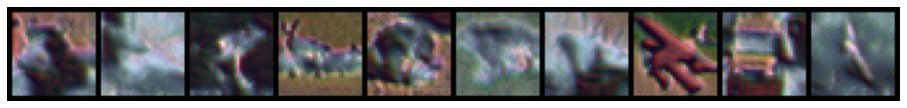
\includegraphics[width=1.4\textwidth]{figures/reconstruction_CIFAR10_RANDOM_NN_epoch_100.png}}
    \caption*{\normalsize{RANDOM NN CC}}
    \rule{0.4\textwidth}{.4pt}
    
    \centerline{\hspace*{8mm}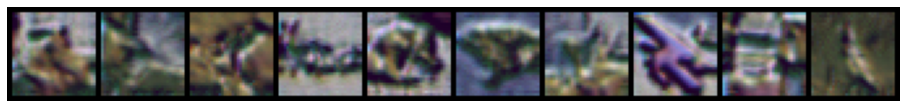
\includegraphics[width=1.4\textwidth]{figures/reconstruction_CIFAR10_RANDOM_NN_CC_epoch_100.png}}
    \caption*{\normalsize{RP}}
    \rule{0.4\textwidth}{.4pt}
    
    \centerline{\hspace*{8mm}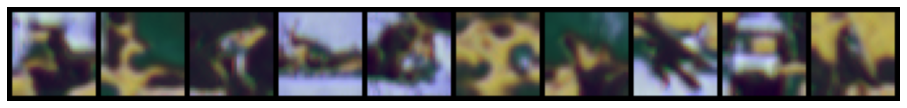
\includegraphics[width=1.4\textwidth]{figures/reconstruction_CIFAR10_RP_epoch_100.png}}
    \caption*{\normalsize{RP CC}}
    \rule{0.4\textwidth}{.4pt}
    
    \centerline{\hspace*{8mm}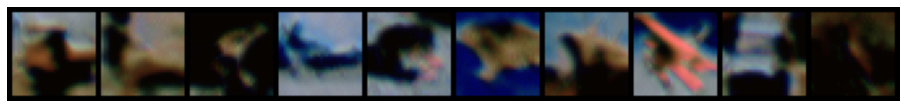
\includegraphics[width=1.4\textwidth]{figures/reconstruction_CIFAR10_RP_CC_epoch_100.png}}
    \caption*{\normalsize{RP ReLU}}
    \rule{0.4\textwidth}{.4pt}
    
    \centerline{\hspace*{8mm}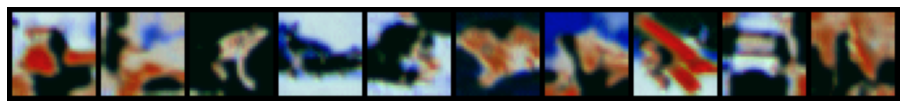
\includegraphics[width=1.4\textwidth]{figures/reconstruction_CIFAR10_RP_ReLU_epoch_100.png}}
    \caption*{\normalsize{RP ReLU CC}}
    \rule{0.4\textwidth}{.4pt}
    
    \centerline{\hspace*{8mm}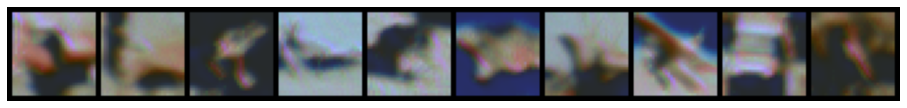
\includegraphics[width=1.4\textwidth]{figures/reconstruction_CIFAR10_RP_ReLU_CC_epoch_100.png}}
    \caption*{\normalsize{COMBINED CC}}
    \rule{0.4\textwidth}{.4pt}
    
    \centerline{\hspace*{8mm}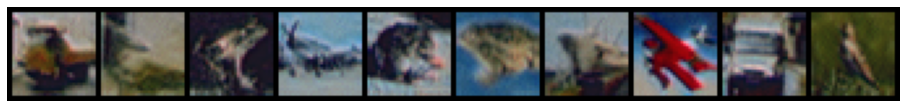
\includegraphics[width=1.4\textwidth]{figures/reconstruction_CIFAR10_COMBINED_CC_epoch_100.png}}
\end{figure}





\chapter{Parameter-Settings}
\label{AppendixParameters}

\begin{table}
\centering
\caption*{\normalsize{\textbf{GMM}}}
\pgfplotstabletypeset[
parameters={\textbf{Data Set}},
every row no 9/.style={
    after row={\\ \textbf{Neural Network} \\ \textbf{Architecture} \\\midrule
        main network: &FCNet4 \\
        verifier network: &FCNet4 \\
    }
},
every row no 10/.style={
    before row={\\ \textbf{Distortion} \\\midrule}
},
every row no 11/.style={
    before row={\multicolumn{2}{l}{\makecell[l]{\\ \textbf{Reconstruction}}} \\\midrule}
},
every row no 12/.style={
    before row={\\ \textbf{Optimization} \\\midrule}
},
]{
$n_{\set A}$ &= 10000
$n_{\set B}$ &= 512
$n_{\set C}$ &= 1024
$d$ &= 20
$C$ &= 10
$n_\textnormal{mode}$ &= 12
$\alpha$ &= 5
$\beta$ &= 20
$\gamma$ &= 3
$\lambda$ &= 3
$\kappa$ &= 0.2
$s_\text{RP}$ &= 256
learning rate &= 0.01
batch size &= 128
$r_\text{crit}$ &= 1
$r_\text{stats}$ &= 0.0005
}
% \label{tab:GMM_params}
\caption{Parameters and specifications of the GMM data set as defined in \ref{sec:datasetgmm}}
\end{table}


%
%   MNIST
%
\begin{table}
% \label{tab:IMAGE_default_params}
\begin{minipage}{0.5\textwidth}
\centering
\caption*{\normalsize{\textbf{MNIST}}}
\pgfplotstabletypeset[
parameters={\textbf{Data Set}},
every row no 3/.style={before row={\\ Properties \\\midrule}},
every row no 5/.style={
    after row={\\ \textbf{Distortion} \\\midrule}
},
every row no 6/.style={
    after row={\\ \textbf{Neural Network} \\ \textbf{Architecture} \\\midrule
        main network: &ResNet20 \\
        verifier network: &ResNet9 \\
    }
},
every row no 7/.style={
    before row={\multicolumn{2}{l}{\makecell[l]{\\ \textbf{Reconstruction Model}}} \\\midrule}
},
every row no 10/.style={
    before row={\\ \textbf{Optimization} \\ \midrule}
},
]{
$n_{\set A}$ &= 60000
$n_{\set B}$ &= 512
$n_{\set C}$ &= 1024
$C$ &= 10
input shape &= (1, 28, 28)
$d$ &= 784
$\kappa$ &= 0.3
$s_\text{width}$ &= 8
$s_\text{depth}$ &= 8
$s_\text{RP}$ &= 512
learning rate &= 0.1
batch size &= 128
$r_\text{crit}$ &= 1
$r_\text{stats}$ &= 0.001
}
\caption{\\ Parameters and specifications of the MNIST data set}
\end{minipage}
%
%   CIFAR10
%
\begin{minipage}{0.5\textwidth}
\centering
\caption*{\normalsize{\textbf{CIFAR10}}}
\pgfplotstabletypeset[
parameters={\textbf{Data Set}},
every row no 3/.style={before row={\\ Properties \\\midrule}},
every row no 5/.style={
    after row={\\ \textbf{Distortion} \\\midrule}
},
every row no 6/.style={
    after row={\\ \textbf{Neural Network} \\ \textbf{Architecture} \\\midrule
        main network: &ResNet34 \\
        verifier network: &ResNet18 \\
    }
},
every row no 7/.style={
    before row={\multicolumn{2}{l}{\makecell[l]{\\ \textbf{Reconstruction Model}}} \\\midrule}
},
every row no 10/.style={
    before row={\\ \textbf{Optimization} \\\midrule}
},
]{
$n_{\set A}$ &= 50000
$n_{\set B}$ &= 512
$n_{\set C}$ &= 1024
$C$ &= 10
input shape &= (3, 32, 32)
$d$ &= 3072
$\kappa$ &= 0.15
$s_\text{width}$ &= 8
$s_\text{depth}$ &= 8
$s_\text{RP}$ &= 512
learning rate &= 0.1
batch size &= 128
$r_\text{crit}$ &= 1
$r_\text{stats}$ &= 10
}
% \decoRule
\caption{\\ Parameters and specifications of the CIFAR10 data set}
%
%
\end{minipage}
\end{table}

% 
% Chapter Template

\chapter{Background}
\label{chap:Background}

\section{Notation}

A \textbf{sample} $\vec z$ is an observation drawn from a joint distribution over the domain $\set Z = \set X \times \set Y$. 
It consists of a tuple $(\vec x, y)$ of an \textbf{input} $\vec x$ and a \textbf{label} $y$. 

\noindent
The input space $\set X$ typically is $\R^d$ and $\set Y$, the set of possible labels, is a set of integers $\{1, \dots, C\}$ for some whole number $C$, also known as the \textbf{number of classes}.

\noindent
A \textbf{bracket-notation} $\finiteset{\, \cdot \,}$ is used to denote the set of all \textit{finite non-empty} subsets.
$\set A = \{\vec z^{(i)}\}_{i=1}^{| \set A |} = \{(\vec x^{(i)}, y^{(i)})\}_{i=1}^{| \set A |} \in \finiteset{\set Z}$ is called a \textbf{data set}. $\set A $ contains \textit{i.i.d.} (independent and identically distributed) samples drawn from some distribution over $\set Z$.
A \textbf{sample batch} or simply \textbf{batch} is a \textit{non-empty} subset thereof.

\noindent
$\mean$ and $\var$ are used to denote the empirical sample mean and variance of the input.
\begin{align*}
    \mean ({\set A}) &= \frac 1 {\lvert \set A \rvert} \sum _{i=1}^{\lvert \set A \rvert} \vec x^{(i)} \; \in \set X \\
    \var ({\set A}) &= \frac 1 {\lvert \set A \rvert} \sum _{i=1}^{\lvert \set A \rvert} (\vec x^{(i)} - \mean ({\set A}))^2 \; \in \set X
\end{align*}


Given a sample batch $\set A$, the set $\set A|_c = \{(\vec x, y) \in \set A \mid y = c\}$ is the subset of $\set A$ \textbf{constrained} to samples of label $c$.


A \textbf{feature-mapping} is any function from input space $\R^d$ to $\R^m$ for some $m$.
A data set to data set mapping is obtained by applying a feature-mapping $\varphi$ to every input. Given a data set $\set A$, and a feature-mapping $\varphi$:
\[
    \varphi(\set A) := \{(\varphi(\vec x), y) \mid (\vec x, y) \in \set A\} \;
    \in \powerset Z
\]



\section{Loss function}
Given two data sets $\set A, \set B$, a \textbf{loss function} or \textbf{objective function} is a function $\loss : \finiteset{\set Z} \times \finiteset{Z} \to \R$ that is \textit{piecewise continuously differentiable} with regard to its inputs.
I. e. where 
\[
    \loss (\set A, \set B) = \loss (
    \,\{(\vec x^{(i)}_{\set A}, y^{(i)}_{\set A})\}_{i=0}^{|\set A|}\,,
    \,\{(\vec x^{(j)}_{\set B}, y^{(j)}_{\set B})\}_{j=0}^{|\set B|}\,) \,,
\]
is piecewise $\mathcal C^1$ with regard to $\vec x^{(i)}_{\set A}$
for all $i=1, \dots, |\set A|$, and $\vec x^{(j)}_{\set B}$ for all $j=1, \dots, |\set B|$.


For a given feature-mapping $\varphi$ that is piecewise $\mathcal C ^1$, it will be defined as follows.
% 
\[
    \loss _{\varphi} (\set A, \set B) = 
    \|\mean ({\varphi (\set A)}) - \mean ({\varphi (\set B)})\| +
    \|\var ({\varphi (\set A)}) - \var ({\varphi (\set B)})\|
\]
% 
A \textbf{class-dependent} loss can be obtained as follows:
\[
    \loss _\varphi ^{\mathcal C} (\set A, \set B) =
    \sum _{\substack{c = 1 \dots C \\ \set A|_c ,\, \set B|_c \neq \emptyset}} 
    \|\mean ({\varphi (\set A|_c)}) - \mean({\varphi (\set B|_c)})\|
    + \|\var ({\varphi (\set A|_c)}) - \var ({\varphi (\set B|_c)})\| 
\]

\subsection{Combinations}
% 
This notion can be extended to a collection of feature-maps [$\varphi_0, \dots, \varphi_n$].
A \textbf{collection} is used to refer to a \textit{non-empty finite} set.
\begin{align*}
    \loss_{[\varphi_1, \dots, \varphi_n]} (\set A, \set B) &= 
    \sum_{i=1}^n \loss_{\varphi_i} (\set A, \set B) \\
    %
    \loss_{[\varphi_1, \dots, \varphi_n]}^{\mathcal C} (\set A, \set B) &= 
    \sum_{i=1}^n \loss_{\varphi_i}^{\mathcal C} (\set A, \set B)
\end{align*}

% \chapter{Objective}
\label{chap:Objective}



%%%%%%%%%%%%%%%%%%%%%%%%%%%%%%%%%%%%%%%%%%%%%%%%
%%%%%%%%%  Section: Reconstruction   %%%%%%%%%%%
%%%%%%%%%%%%%%%%%%%%%%%%%%%%%%%%%%%%%%%%%%%%%%%%


\section{Reconstruction}
\label{sec:Reconstruction}

\begin{figure}[h]
    
% RECONSTRUCTION GRAPH
\begin{tikzpicture}[node distance=1cm and 1.7cm, auto]
%%Nodes

\node (D) [minimum height=3.5cm] {\distribution};
\node [above of= D, align=center, yshift=0.7cm] {data set \\ distribution};

\node (A) [node, right= 1cm of D, fill=red!7, yshift=1.5cm] {\textbf{target} \\ $\set A$};
\node (B) [node, right= 1cm of D, yshift=-1.5cm] {\textbf{original} \\ $\set B_\text{true}$};

\node (Bp) [node, right= of B, fill=blue!3] {perturbed \\ \textbf{source} \\ $\set B$}; %\\ $\set B = \delta (\set B_\text{true})$};
\node (Br) [node, right= of Bp, fill=blue!7] {\textbf{reconstructed} \\ $\rho (\set B)$};


%%Arrows
\draw [arrow, dashed, thin] (D) -- (A.190);
\draw [arrow, dashed, thin] (D) -- (B.170);


\draw [arrow, dashed, thin] (B) -- (Bp) 
node (Pert) [midway, function, dashed] {$\delta$};
\draw [linestart] (Bp) -- (Br) 
node (Rec) [midway, function, draw=blue, fill=white] {$\rho$};
\node [fill=white, below= 0cm of Rec] {\color{blue} \footnotesize optimize};
\node [fill=white, below= 0cm of Pert] {\footnotesize \textit{unknown}};


% \draw [dashed] (Rec) to [out=245, in=115] (Rec2);

\node (Net) [function, thick, minimum width= 1cm, above right= -0cm and 3.1cm of A] {$\varphi$};
\node [above right=-0.2cm and 0cm of Net] {\small feature-map};
\node (Loss) [function, thick, above= 1.5cm of Net] {Loss};

\pgfmathtruncatemacro{\OutL}{110}
\pgfmathtruncatemacro{\OutM}{95}
\pgfmathtruncatemacro{\OutR}{75}
\pgfmathtruncatemacro{\InL}{360-\OutL}
\pgfmathtruncatemacro{\InM}{360-\OutM}
\pgfmathtruncatemacro{\InR}{360-\OutR}

\draw [lineend] (Net.\InL) to [corner connect h=-0.7cm] (A.east);
\draw [arrowend] (Net.\OutL) to [out=90, in=270] (Loss.260);

\draw [line] (Net.\InM) to [rect connect h=-0.7cm] (Br.100);
\draw [arrowend] (Net.\OutM) to [out=90, in=270] (Loss.260);

\draw [line, blue] (Net.\InR) to [rect connect h=-0.4cm] (Br.80);
\draw [lineend, blue, connect v] (Net.\OutR) to (Loss.south);
\draw [arrowend, blue, connect h] (Br.192) to (Rec.east);

\path (Net.\OutL) -- node[midway, above= 0.15cm, sloped] {\small statistics}(Loss.260);
% \node [above= 0.5cm of Net, fill=white] {\footnotesize optimize};
% \draw [arrow, Mahogany, thin, bend left=20] (A) to node[near end, above] {\footnotesize trained} (Net);

\node [above= 1cm of B, yshift=-1.5cm] {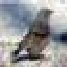
\includegraphics[]{figures/CIFAR10_example.pdf}};

\end{tikzpicture}




% % RECONSTRUCTION GRAPH
% \begin{tikzpicture}[node distance=1cm and 1.7cm, auto]
% %%Nodes

% \node (D) [minimum height=3.5cm] {\distribution};
% \node [above of= D, align=center, yshift=0.7cm] {data set \\ distribution};

% \node (A) [node, right= 1cm of D, fill=red!7, yshift=1.5cm] {\textbf{target} \\ $\set A$};
% \node (B) [node, right= 1cm of D, yshift=-1.5cm] {\textbf{original} \\ $\set B_\text{true}$}

% \node (Bp) [node, right= of B, fill=blue!3] {perturbed \\ \textbf{source} \\ $\set B$}; %\\ $\set B = \delta (\set B_\text{true})$};
% \node (Br) [node, right= of Bp, fill=blue!7] {\textbf{reconstructed} \\ $\rho (\set B)$};


% %%Arrows
% \draw [arrow, dashed, thin] (D) -- (A.190);
% \draw [arrow, dashed, thin] (D) -- (B.170);


% \draw [arrow, dashed, thin] (B) -- (Bp) 
% node (Pert) [midway, function, dashed] {$\delta$};
% \draw [linestart] (Bp) -- (Br) 
% node (Rec) [midway, function, draw=blue, fill=white] {$\rho$};
% \node [fill=white, below= 0cm of Rec] {\color{blue} \footnotesize optimize};
% \node [fill=white, below= 0cm of Pert] {\footnotesize \textit{unknown}};


% % \draw [dashed] (Rec) to [out=245, in=115] (Rec2);

% \node (Net) [function, thick, minimum width= 1cm, above right= -0cm and 3.1cm of A] {$\varphi$};
% \node [above right=-0.2cm and 0cm of Net] {\small feature-map};
% \node (Loss) [function, thick, above= 1.5cm of Net] {loss};

% \pgfmathtruncatemacro{\OutL}{110}
% \pgfmathtruncatemacro{\OutM}{95}
% \pgfmathtruncatemacro{\OutR}{75}
% \pgfmathtruncatemacro{\InL}{360-\OutL}
% \pgfmathtruncatemacro{\InM}{360-\OutM}
% \pgfmathtruncatemacro{\InR}{360-\OutR}

% \draw [lineend] (Net.\InL) to [corner connect h=-0.7cm] (A.east);
% \draw [arrowend] (Net.\OutL) to [out=90, in=270] (Loss.260);

% \draw [line] (Net.\InM) to [rect connect h=-0.7cm] (Br.100);
% \draw [arrowend] (Net.\OutM) to [out=90, in=270] (Loss.260);

% \draw [line, blue] (Net.\InR) to [rect connect h=-0.4cm] (Br.80);
% \draw [lineend, blue, connect v] (Net.\OutR) to (Loss.south);
% \draw [arrowend, blue, connect h] (Br.192) to (Rec.east);

% \path (Net.\OutL) -- node[midway, above= 0.15cm, sloped] {\small statistics}(Loss.260);
% % \node [above= 0.5cm of Net, fill=white] {\footnotesize optimize};
% % \draw [arrow, Mahogany, thin, bend left=20] (A) to node[near end, above] {\footnotesize trained} (Net);


% \end{tikzpicture}


    \caption{Overview}
    \centering
\end{figure}

This section describes the main objective of the task.
The goal is to learn an inverse transformation to the unknown $\delta$.
The way this is achieved is by maximizing similarity between the distributions of a source data set $\set B$
and a target data set $\set A$ in an appropriate feature-space $\phi$.
The goal of maximizing similarity in feature-space is addressed by formulating a loss function
that minimizes simple statistics, such as the mean and variance of the dataset.

Example application:
A neural network might be well adjusted to a target distribution, 
though under-perform when presented with samples that don't follow the original distribution
and exhibit different statistics to which the neural network was not adjusted to.
To combat this problem, a method for readjusting the inputs is introduced.
The basic idea is that the data is mapped to a feature-representation.
In this feature-space, simple statistics, such as the mean and variance are recorded
for both, a source data set $\set B$ and a target data set $\set A$.
Although, the source is first sent through a re-adjustment function $\rho$ that is
then tuned to minimize the similarity-loss of the two data sets.
This is done via a differentiable loss, or objective function that minimizes the difference in statistics.



\subsection{Problem Formulation}
Given: feature-map $\varphi$, target data set $\set A$ (or $\varphi(\set A)$ statistics), and a perturbed data set $\widetilde {\set B}$

\[
    \min_{\rho \in \mathcal{F}} \loss _\varphi (\set A, \rho(\widetilde{\set B})) \,,
\]
where $\mathcal F$ is a pre-defined set of functions.






%%%%%%%%%%%%%%%%%%%%%%%%%%%%%%%%%%%%%%%%%%%%%%%%
%%%%%%%%%%   Section: Inversion    %%%%%%%%%%%%%
%%%%%%%%%%%%%%%%%%%%%%%%%%%%%%%%%%%%%%%%%%%%%%%%


\section{Inversion}
\label{sec:Inversion}

\begin{tikzpicture}[node distance=1.3cm and 1.4cm, auto]

%%Nodes
\node (D) [minimum height=3.5cm] {\distribution};
\node [above of= D, align=center, yshift=0.2cm] {data set \\ distribution};

\node (N) [below= -0.5cm of D, minimum height=3.5cm] {\noise};
\node [above of= N] {random noise};

\node (B) [node, right= of N, fill=blue!7, draw=blue, thick] {\textbf{Source} \\ $\set B$};
\node (A) [node, right= of D, fill=red!7] {\textbf{target} \\ $\set A$};

\path (A) -- (B) node (Mid) [midway] {};
\node (Net) [function, thick, minimum width=1cm, right= of Mid, xshift=1.2cm] {$\varphi$};
\node [below right= 0.1cm and -1.2cm of Net] {\small feature-map};
\node (Loss) [function, thick, right= of Net] {loss};

%%Arrows
% \pgfmathtruncatemacro{\InL}{160}
% \pgfmathtruncatemacro{\InM}{175}
% \pgfmathtruncatemacro{\InR}{195}
% \pgfmathtruncatemacro{\OutL}{360-\InL}
% \pgfmathtruncatemacro{\OutM}{360-\InM}
% \pgfmathtruncatemacro{\OutR}{360-\InR}
\pgfmathtruncatemacro{\OutL}{20}
\pgfmathtruncatemacro{\OutM}{5}
\pgfmathtruncatemacro{\OutR}{-15}
\pgfmathtruncatemacro{\InL}{180-\OutL}
\pgfmathtruncatemacro{\InM}{180-\OutM}
\pgfmathtruncatemacro{\InR}{180-\OutR}

\draw [arrow, dashed, thin] (D) -- (A);
\draw [arrow, dashed, thin] (N) -- (B);

\draw [linestart] (A.east) to [rect connect v=1cm] (Net.\InL);
\draw [arrowend] (Net.\OutL) to[out=0, in=180]  (Loss.170);

\draw [linestart] (B.15) to [rect connect v=1cm] (Net.\InM);
\draw [arrowend] (Net.\OutM) to[out=0, in=180] (Loss.170);

\draw [arrowend, blue] (Net.\InR) to[out=180, in=0, rect connect v=-0.5cm] (B.-5);
\draw [lineend, blue, connect h] (Net.\OutR) to (Loss.west);
\node [below= 0cm of B, yshift=-0cm] {\color{blue} \footnotesize optimize};

\path (Net) -- (Loss) node [above=0.3cm, midway] {\small statistics};
% \draw [arrow, Mahogany, thin, bend left=30] (A.20) to [out=40, in=140] node[above, sloped] {\footnotesize trained} (Net);

\node [below= 0cm of A] {\fbox{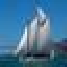
\includegraphics[]{figures/CIFAR10_example_3.pdf}}};

\end{tikzpicture}



The second part of this work is concerned about what kind of data may be recovered from 
having knowledge of the statistics of a data set.
For this task, the goal is to modify the source data set $\set B$ to more closely resemble
the target data set $\set A$ only given the statistics of data set $\set A$.
The source data set $\set B$ is in a first step, initialized by random noise.
Then, by performing gradient descent on the loss function, the source itself is optimized.



\subsection{Objective}
Given: $\varphi$, $\set A$ (or $\varphi(\set A)$ statistics), 
fixed size $n_{\set B}$, target labels $\{y^{(i)}\}_{i=1}^{n_{\set B}}$.
\[
    \min_{\set B \in \finiteset {\set Z}} \loss _\varphi (\set A, \set B) \comma{where} 
    \set B = \{(\vec x^{(i)}, y^{(i)})\}_{i=1}^{n_{\set B}}
\]
    


\subsection{Inversion Evaluation}
The result of the optimization process can be evaluated by calculating the accuracy obtained by $\Phi$. 
Though, since $\Phi$ was used in the optimization process, it will likely display heavy bias to what it believes is a correctly classified sample.
For this sake, another neural network $\Phi_{\text{ver}}$ can be employed, which has been separately trained on either $\set A$ or another data set. 

%Though, practice has shown that a very small portion of $\set A$ is only needed to obtain a close-enough guess at the true statistics of $\set A$.




% 
\chapter{Experiments}
\label{chap:Experiments} 

\section{Methods}

The success of the reconstruction largely depends on the representation of the data
after the feature-map is applied.
Although, assuming that the data distribution of the data can be accurately described
by a mean and a variance is a strong assumption.
More sophisticated ways of modeling data distributions exist
\XXX{insert some}
, yet mean and variance were chosen due to their simplicity in evaluation and computing of the gradients.

The feature-map will ideally "disentangle" the data space to enable 
simple statistics to capture the complexity of the data set.

It is hypothesized that neural networks "disentangle" the input space in order to end up with an efficient feature-representation in its later layers.
(This becomes more apparent when one imagines that most neural networks must learn to classify by linearly separating its features obtained from the previous to last layer.)


For assessing the efficacy of the ability to capture the data distribution by
the statistics of the intermediary representations in a neural network,
several different mappings or collections of mappings will be compared. 

For every method there exists a class-dependent variant.
\subsection{Neural Network}

A \textbf{neural network} $\Phi$ is a function that maps an input $\vec x \in \R^d$ to a label $y$.
Normally, in classification tasks, where one hopes to assign a label to an input, the output of a neural network is a C-dimensional vector..
\XXX{maybe not, logit; DEF}. 
A \textbf{multi-layer perceptron} (MLP) is a special type of neural network. Throughout this work, when referring to a neural network, a multi-layer perceptron is meant. A MLP is a composition of functions $\Phi_i$, also called \textbf{layers} that successively act on the outputs $\vec h$ of the previous layer, called \textbf{activations} or \textbf{hidden states}. 
The last layer is referred to as the \textbf{logits-layer}. 
The predicted output label $\hat y$ is normally obtained by returning the index of the maximum value in the logits-layer, thus $\R^{\textnormal L} = \R^C$.
In a plain \textbf{fully-connected} neural network, the layers are each made up of an affine linear transformation and a non-linear activation function.

Formally, a fully-connected neural network of layer depth L is described as:

\[
    \Phi = \Phi_\text{L} \circ \ldots \circ \Phi_1
\]
\[
    \vec h_\ell = (\Phi_\ell \circ \ldots \circ \Phi_1) (\vec x) =
    \Phi_\ell(\vec h_{\ell-1}) \in \R^{d_\ell}
\]
$\Phi_\ell$ then, is a mapping from $\R^{d_{\ell-1}}$ to $\R^{d_\ell}$. 
The space of a hidden state $\vec h$ is called a \textbf{feature-space}.
The input $\vec x$ is also referred to as $\vec h_0$ and $\R^{d_0} := \R^d$.

\[
    \Phi_\ell(\vec h) = \sigma (\vec W \vec h + \vec b) \comma{where}
    \vec W \in \R^{d_\ell \times d_{\ell-1}} \comma{and}
    \vec b \in \R^{d_\ell}
\]
The affine linear transformation is made up of a \textbf{weight matrix} $\vec W$ and a \textbf{bias} $\vec b$.
The non-linear activation function $\sigma$ is often one of \textit{ReLU} (Rectified Linear Unit), \textit{tanh} or \textit{softmax}. The former two are mappings from $\R$ to $\R$ that are applied element-wise.




\subsection{Neural Network - last layer}

Given a neural network $\Phi$ of depth L..
A feature-mapping can be obtained by mapping inputs to the second-to-last layer.
Generally, this is seen as a layer with the best feature representation? source?


\[
    \varphi : \R^d \to \R^{d_\textnormal{L-1}} = (\Phi_\textnormal{L-1} \circ \dots \circ \Phi_1)
\]
\subsection{Neural Network - all layers}
All hidden states of the neural network are used to produce a collection of mappings [$\varphi_0, \dots, \varphi_\text{L}$].
\begin{alignat*}{2}
    \varphi_\ell &: \R^d \to \R^{d_\ell} &&= (\Phi_\ell \circ \dots \Phi_1) \quad
    \text{for $\ell = 1, \dots$, L - 1} \\
    \varphi_\textnormal{L} &: \R^d \to \R^d &&= \Id
\end{alignat*}





\subsection{Random Projections}
The method of projecting the input to the hidden representations of a neural network will be contrasted with taking $n$ random linear projections.
A random projection is a linear mapping $r: \R^d \to \R$
It is created by choosing a normalized random vector $\vec v \in S^{d-1} = \{\vec x \in \R^d : \|\vec x\| = 1\}$.
It is a simple linear projection on to the one-dimensional subspace defined by the vector $\vec v$.
\[
    r(\vec x) = \vec v ^\top \vec x
\]
By choosing a total of n random vectors $\{v_1, \dots, v_n\}$ one obtains a linear mapping $R: \R^d \to \R^n$:
\[
    R(\vec x) = \vec V \vec x =
    \begin{bmatrix}
        - \vec v_1 ^\top - \\
        \vdots \\
        - \vec v_n ^\top - \\
    \end{bmatrix}
    \vec x =
    \begin{bmatrix}
        \vec v_1 ^\top \vec x \\
        \vdots \\
        \vec v_n ^\top \vec x \\
    \end{bmatrix}
\]
%
The loss function $\loss_R$ stays as was defined before.
Though it might be more reasonable to have the projection centered around a more suitable position than to just project from the origin, in order to obtain better scaled values.
% 
\[
    R_{\vec o} (\vec x) = \vec V (\vec x - \vec o) \,,
\]
where $\vec o \in \R^d$ is the new origin of the projection. Although, practically one often works with normalized data anyhow..
The class-dependent variant can be modified to select an origin $\vec o_c$ for each class $c$.
% 
\begin{align*}
    \loss _R ^{\mathcal C} (\set A, \set B) &=
    \begin{aligned}[t]
        \sum _{\substack{c = 1 \dots C \\ \set A|_c ,\, \set B|_c \neq \emptyset}} 
        \|\mean ({R_{\vec o_c} (\set A|_c)}) - \mean ({R_{\vec o_c} (\set B|_c)}) \| \\
        {} + \|\var ({R_{\vec o_c} (\set A|_c)}) - \var ({R_{\vec o_c} (\set B|_c)}) \| 
    \end{aligned}
\end{align*}

The idea is to set the origin to be at the center of each class of the target data set $\set A$. $\vec o_c = \mean ({\set A|_c})$
This way we can ensure a balanced output..



\subsection{Random Projections ReLU}
To further explore the influence of the non-linear activation functions contained within the network,
one can combine the previous method with adding an activation function, in this case the ReLU.
% 
\[
    R_{\vec o}^+ (\vec x) = (\vec V (\vec x - \vec o))^+ \,,
\]
where $(\,\cdot\,)^+ :\R^n \to \R^n$ is the projection onto the positive orthant. It applies $\max(0, \cdot)$ element-wise.

Since ReLUs have a bias parameter that shifts the threshold where an input can pass, this will also be incorporated.
This bias parameter usually doesn't come from the ReLU itself, but is incorporated in the previous layer's affine transformation.
\[
    R_{\vec o}^{\vec b} (\vec x) = (\vec V (\vec x - \vec o) + \vec b)^+ \,,
\]
where $\vec b \in \R^d$ is the bias. For a target dataset $\set A$, it is chosen as $\vec b \sim \mathcal N(\boldsymbol \mu, \textnormal{diag}(\boldsymbol \sigma ^2))$, 
where $\boldsymbol \mu = \mean ({R_{\vec o}(\set A)})$ and $\boldsymbol \sigma ^2 = \var ({R_{\vec o}(\set A)})$.

The class-dependent variant can again make use for more suited origins of projection $\vec o_c$ and individual biases $\vec b_c$.
$\vec b_c$ is chosen at random to be centered around the output $\sim \mathcal N(\boldsymbol \mu_c, \textnormal{diag}(\boldsymbol \sigma _c^2))$, 
where $\boldsymbol \mu_c = \mean ({R_{\vec o}(\set A|_c)})$ and $\boldsymbol \sigma_c ^2 = \var ({R_{\vec o}(\set A|_c)})$ for all non-empty $\set A|_c$.
% 
\begin{align*}
    \loss _{R^+} ^{\mathcal C} (\set A, \set B) &=
    \begin{aligned}[t]
        \sum _{\substack{c = 1 \dots C \\ \set A|_c ,\, \set B|_c \neq \emptyset}} 
        \|\mean ({R_{\vec o_c}^{\vec b_c} (\set A|_c)}) - \mean ({R_{\vec o_c}^{\vec b_c} (\set B|_c)})\| \\
        {} + \|\var ({R_{\vec o_c}^{\vec b_c} (\set A|_c)}) - \var ({R_{\vec o_c}^{\vec b_c} (\set B|_c)}) \| 
    \end{aligned}
\end{align*}

\subsection{Randomly initialized Neural Network}
To study the importance of an optimized feature-representation of a trained neural network, 
the same neural network model with randomly initialized parameters will be evaluated and compared.

\subsection{Combinations}
Combinations of all previously defined losses and feature-maps can be made. In particular, the combination of all neural network layers and random projections will be examined in order to report any improvement.


\section{Data sets}
\subsection{Gaussian mixture models}
A Gaussian mixture dataset comprising $C$ classes, each of which is made up of $n_\text{mode}$ clusters or modes of multivariate Gaussian Normal distributions.
\begin{align}
\label{eqn:gmmdistr}
    p(\, \vec x \mid \boldsymbol \theta, c \,) = \frac 1 {n_\text{mode}} \sum _{i=0}^n
    \mathcal N (\vec m_c + \boldsymbol \mu_c^{(i)}, \boldsymbol \Sigma_c^{(i)})
\end{align}
$\vec m_c \sim \mathcal N (\vec 0, \gamma \vec I)$ and
$\boldsymbol \mu_c^{(i)} \sim \mathcal N (\vec 0, \lambda \vec I)$ and
$\vec \Sigma_c^{(i)}$ is generated by choosing $d$ eigenvalues $\vec e \sim \mathcal U(\alpha, \beta)$, $\alpha, \beta > 0$ and 
by sampling a random orthogonal matrix $\vec Q$. The specifics of $\Sigma$ are not too important.
\XXX{elaborate?}
\begin{align*}
    \vec \Sigma = \vec Q^\top \text{diag}(\vec e) \vec Q
\end{align*}
For a given data set size N and parameters $\alpha, \beta, \gamma, \lambda$; N data points are generated by uniformly sampling from all classes to obtain a label, then the input will be sampled according to \eqnref{eqn:gmmdistr}.

\subsection{MNIST}
MNIST is a dataset of xxx black-and-white images of handwritten digits from 0 to 9. 
Each Image is made up of 28x28 pixels, total 784.

\subsection{CIFAR-10}
CIFAR10 contains xxx colored images from 10 non-overlapping categories.
Each Image has 3 Channels and 32x32 pixels, totaling a dimension of 3072.



\subsection{Evaluation}

\begin{tikzpicture}[node distance=1cm and 1.7cm, auto]

\node (A) [node, fill=red!7] {\textbf{Target} \\ $\set A$};
\node (B) [node, below= of A] {\textbf{original} \\ $\set B_\text{true}$};
\node (C) [node, below= 2.2cm of B, fill=blue!0] {\textbf{Validation} \\ $\set C_{true}$};

\node (Bp) [node, right= of B, fill=blue!2] {perturbed \\ \textbf{Source} \\ $\set B$};
\node (Br) [node, right= of Bp, fill=blue!7] {\textbf{reconstructed} \\ $\rho^* (\set B)$};


\draw [arrow, dashed, thin] (B) -- (Bp) node (Pert) [midway, function, dashed] {$\delta$};
\draw [arrow] (Bp) -- (Br) node (Rec) [midway, function] {$\rho^*$};
\node [fill=white, below= 0cm of Pert] {\footnotesize \textit{unknown}};
\node [fill=white, below= 0cm of Rec] {\footnotesize \textit{learned}};


\node (Net) [function, fill=gray!5, above= of Br] {Neural \\ Network};
\node (vNet) [function, fill=gray!5, right= of Net] {verification \\ Neural \\ Network};

\draw [arrow, Mahogany, thin, bend left=20] (A) to (Net);
\draw [arrow, Mahogany, thin, bend left=20] (A) to node[below] {\footnotesize trained} (vNet);
\draw [arrow, Blue, thin] (Net.210) to[bend right=20] node [midway, above, sloped] {\footnotesize optimized} (Rec.north);

\node (Cp) [node, right= of C, fill=blue!0] {\textbf{perturbed} \\ $ {\set C}$};
\node (Cr) [node, right= of Cp, fill=blue!0] {\textbf{reconstructed} \\ $\rho ^*( {\set C})$};


\draw [arrow, dashed, thin] (C) -- (Cp);
\draw [arrow] (Cp) -- (Cr);

\draw [arrow, dashed, thin] (C) -- (Cp) node (Pert) [midway, function, dashed] {$\delta$};
\draw [arrow] (Cp) -- (Cr) node (Rec) [midway, function] {$\rho^*$};

\draw [arrow, <->, thin, OliveGreen] (Br.south) to [rect connect h=-0.75cm] (B.south);
\draw [arrow, <->, thin, OliveGreen] (Cr.north) to [rect connect h=0.75cm] (C.north);

\path (Br.east) to [out=0, in=270]  node [near end, OliveGreen, xshift=0.1cm] {accuracy} (vNet.265);
\draw [arrow, thin, OliveGreen] (Br.east) to [out=0, in=320] (Net.315);
\draw [arrow, thin, OliveGreen] (Cr.east) to [out=0, in=320] (Net.325);
\draw [arrow, thin, OliveGreen] (Cr.east) to [out=0, in=270] (vNet.south);


\node [OliveGreen] at ($(Bp)!0.5!(Cp)$) {IQA metrics};

\node [below= 1.5cm of Pert] (Id) {Id};
\path (Id) -| node[anchor=center] (Idr) {$\hat {\Id}$} (Rec);
\draw [arrow] (Id) -- 
node[near start, xshift=0.2cm, function] {$\delta$} 
node[near end, xshift=-0.2cm, function] {$\rho^*$} (Idr);
\draw [arrow, <->, thin, OliveGreen] (Idr.south) to [rect connect h=-0.6cm] (Id.south);
\node [OliveGreen, yshift=-1.2cm] at ($(Id)!0.5!(Idr)$) {rel. error};
% \node [circle, fill=blue] at (Idr){};
% \draw (0,0)|-node{mid}(2,3);
% \node [below= 1cm of Rec] {};
% \node (Cbelow) [below= of Cp] {EEE};
% \draw [arrow, dashed, thin] (C) -- (Cp) node (Pert) [midway, function, dashed] {$\delta$};
% \draw [arrow] (Cp) -- (Cr) node (Rec) [midway, function] {$\rho^*$};

\end{tikzpicture}


For the main reconstruction task, 
five metrics will be studied to determine a methods success (along with visual appeal).
For one, the accuracy of the reconstructed data set will be measured by the neural network.
The relative l2-error, the peak signal-to-noise ratio, the accuracy of the neural network and the accuracy on a verifier network.
Alongside, a validation data set $\set C$ will measure generalization of the found reconstruction $\rho$ to a data set to which it was not optimized for.
Since the original neural network was also used in the optimization process, a verifier network $\Phi_{\text{ver}}$ will be used as a second evaluation of the accuracy.

If the perturbation $\delta$ is known, then one can calculate the \textbf{relative error} of the identity vectors. 
\begin{equation}
\label{eqn:relerror}
    \varepsilon_F = \frac {\|\widehat {\vec I_d} - \vec I_d\|_F} {\|\vec I_d\|_F} \,,
\end{equation}
where $\widehat {\vec I_d} = \begin{pmatrix} \rho (\delta (\vec e_1), \dots, \rho (\delta (\vec e_d) \end{pmatrix}$ and $\vec e_i$ is the i-th unit vector.

Then \eqnref{eqn:relerror} becomes
\[
    \varepsilon_F = \frac 1 {\sqrt d} \sqrt{ \sum_{i=0}^d \|\rho (\delta (e_i)) - e_i)\|_2^2}
\]

The \textbf{PSNR} (peak signal-to-noise ratio) between $\vec x$ and $\vec y$ is calculated as follows.
\[
    PSNR(\vec x, \hat {\vec x}) = 20 \log_{10} \left (\frac {\max_i(\vec x_i)} {\|\vec x-\hat {\vec x}\|_2} \right )
\]
It is a common measure of image quality when assessing image compression algorithms and is measured in decibels db.
It is similar to the relative error in that it uses the mean-squared error, though it assessed on the images directly.
For a batch of images, the score is averaged over the images to give a mean PSNR score.

\subsection{Results}

% 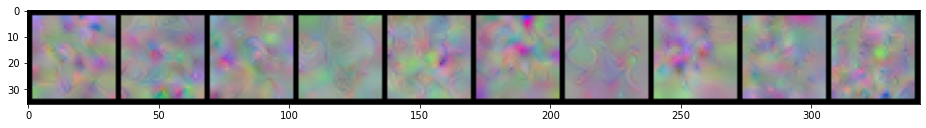
\includegraphics[width=\textwidth]{figures/INVERSION_CIFAR10_NN_0.png}



% \documentclass{article}
% \usepackage{graphicx}

% \ifluatex
%   \directlua{
%     tex.enableprimitives('', {'luaescapestring'})
%   }
%   \newcommand*{\Download}[2]{%
%     \IfFileExists{#1}{%
%     }{%
%       \directlua{
%         local io = require('io')
%         local http = require('socket.http')
%         local ltn12 = require('ltn12')
%         local file_name = '\luaescapestring{#1}'
%         local url = '\luaescapestring{#2}'
%         texio.write_nl('Downloading: ' .. file_name)
%         texio.write_nl('')
%         http.request{
%           url=url,
%           sink=ltn12.sink.file(io.open(file_name, 'w'))
%         }
%       }%
%     }%
%     \edef\DownloadFile{#1}%
%   }
% \else
%   \newcommand*{\Download}[2]{%
%     \IfFileExists{#1}{%
%     }{%
%       \immediate\write18{%
%         wget -O "#2" "#1"%
%       }%
%     }%
%     \edef\DownloadFile{#1}%
%   }%
% \fi

% \begin{figure}
% \centering
% \Download{profile-pics-16.jpg}{%
%     https://cdn.mos.cms.futurecdn.net/42E9as7NaTaAi4A6JcuFwG-970-80.jpg%
% }
% \includegraphics{\DownloadFile}
% \end{figure}
% \section{Results}

\subsection{Quantitative Results}

\pgfplotstableset{
col sep = comma,
string replace*={_}{\textsubscript},
every head row/.style={before row=\toprule,after row=\midrule},
every last row/.style={after row=\bottomrule},
every column/.style={column type=l, precision=1, zerofill},
columns={[index]0, [index]1, [index]2, [index]3, [index]4, [index]5, [index]6},
display columns/0/.style={column name=\textbf{Method}, column type=l, string type},
display columns/1/.style={column name=\textbf{Accuracy} [\%], multiply with=100},
display columns/2/.style={column name=\makecell{validation \\ \textbf{Accuracy}} [\%], column type=l, multiply with=100},
display columns/3/.style={column name=\makecell{verifier \\ \textbf{Accuracy}} [\%], column type=l, multiply with=100},
display columns/4/.style={column name=\textbf{l2-error}},
display columns/5/.style={column name=\textbf{PSNR}},
display columns/6/.style={column name=\textbf{SSIM} [\%], column type=l, multiply with=100},
}
\pgfplotstabletypeset{figures/reconstruction_CIFAR10_baseline.csv}
\pgfplotstabletypeset{figures/reconstruction_CIFAR10_results.csv}


% \chapter{Introduction}

\label{Introduction}

Neural networks designed for a classification task typically map inputs coming from a very high-dimensional space to a rather low-dimensional space - the space of possible classes.
$$
x \in \R^n,\ y \in \R^m ,\ n \gg m
$$
$$\phi (x) = y
$$
Given the nature of such a task, this forward process typically incurs in a huge loss of information. When $n > m$ and the data is not contained in some lower-dimensional submanifold, then the restriction of the map $\phi$ to the data manifold can not be bijective and therefore not invertible. 
Thus, given only the output, it is generally not possible to recover the input.
Typically, this transformation of the input to more abstract, meaningful features, along with the resulting compression is desired. Yet, the inverse problem of accurately modeling the posterior distribution $p(x|\;y)$ or an approximation thereof is an active area of research with many applications.
Such advantages of invertibility can be more efficient training, knowledge distillation in teacher-student networks, but also most notably, interpretability of a neural network's decision process - a big concern in security-related fields such as medical sciences, autonomous vehicles and face-recognition. 

Some recent work in this area are \textit{Invertible Neural Networks} \citep{ardizzone2018analyzing} , \textit{Glow: Generative Flow with Invertible 1x1 Convolutions} \citep{kingma2018glow} and \textit{Invertible Residual Networks} \citep{behrmann2018invertible}. The methods used vary from noise-optimization, direct parametrization to solving fixed-point iterations.

For the sake of interpretability, it is often enough to be able to sample from the posterior distribution.
The method that will be further examined in this work is an iterative refinement-process that optimizes random noise or an existing image to meet some criterion. This method was made popular by the computer vision program \textit{DeepDream} \citep{DeepDream} and later further improved on by \textit{DeepInversion} \citep{DeepInversion}.

% \include{Chapters/Chapter1}
% % Chapter Template

\chapter{Feature Regularization} % Main chapter title

\label{Chapter2} % Change X to a consecutive number; for referencing this chapter elsewhere, use \ref{ChapterX}

%----------------------------------------------------------------------------------------
%	SECTION 1
%----------------------------------------------------------------------------------------

The basic idea used for dataset-reconstruction will be illustrated using a neural network trained for a simple classification task on a two-dimensional toy dataset. The same principle can be applied to image-classification networks, although intuition does not always hold in the very high-dimensional setting.

\begin{figure}
\centering
\includegraphics[width=0.5\textwidth]{Figures/toy_dataset.png}
\decoRule
\caption{toy dataset}
\label{fig:toy_dataset}
\end{figure}

%Given a dataset consisting of multiple classes, each with distinct features (as seen in \ref{fig:toy_dataset}), a neural network designed for the task of classification can generally (given that the  network is expressive enough) be trained to attain a high accuracy for this task.

\begin{figure}
\centering
\includegraphics[width=0.5\textwidth]{Figures/toy_dataset_contour.png}
\decoRule
\caption{prediction by the neural network}
\label{fig:toy_dataset_contour}
\end{figure}

In the case of a two-dimensional dataset (as seen in \ref{fig:toy_dataset}), the predicted outcome of the neural network for any given point and the decision boundary can easily be visualized, as shown in \ref{fig:toy_dataset_contour}.
Here, a fully-connected neural network with two hidden layers of dimensions 8 and 6 was trained using the cross-entropy loss function to achieve a 100\% correct classification rate.

A method for reconstructing a data-point of a certain target-class $\hat y$, given only the neural network, is to start with a randomly initialized point in the input-space and then incrementally tweak it to maximize the neural network's response for the given class $\hat y$. In the same fashion as updating the weights of the network by gradient descent to minimize the error, the point can be updated instead to reach a lower classification-error.
This corresponds to minimizing the loss $\mathcal L$, given $\hat y$  with respect to the input $x$.
$$\min_x \mathcal L (x,\hat y)
$$

\begin{figure}
\centering
\includegraphics[width=0.5\textwidth]{Figures/toy_dataset_invert.png}
\decoRule
\caption{dataset-reconstruction}
\label{fig:toy_dataset_invert}
\end{figure}

The path such a data point might undertake in the optimization-process is shown in \ref{fig:toy_dataset_invert}.
In this setting, in order to gain further insight, the loss that is being optimized for can be plotted for each class individually. The resulting scalar-field is shown in  \ref{fig:toy_dataset_loss_landscape} and will be referred to as the \textit{loss-landscape}.

\begin{figure}
\centering
\includegraphics[width=\textwidth]{Figures/toy_dataset_loss_landscape.png}
\decoRule
\caption{loss-landscape}
\label{fig:toy_dataset_loss_landscape}
\end{figure}

Through this visualization it becomes clear that the points in \ref{fig:toy_dataset_invert} are moving toward local minima in the loss-landscape.
Some issues that are already foreseeable with this method is that the resulting end-points can (and in the most cases will) be chaotic with respect to the initialization. Points that are initially "close" can result in very different outcomes. It is also not immediately clear how many iteration-steps to perform or what criterion for stopping to meet when reconstruction is performed.
Another problem could be that points might "trail off" from the dataset-cluster or that points starting further away might keep their distance during the optimization-process. These points might be given a high score for belonging to the target-class by the network, yet they might not share the same statistics as "natural" data-points. This is seen in \ref{fig:toy_dataset_invert} as the reconstructed points don't end up near the clusters.

A way to combat this is to enforce similar statistics as those of the original dataset by including a regularization-term $\mathcal R$. In order to perform this, statistics, such as the mean and variance need to be tracked as additional parameters of the network (this can be done during training-time or once after training).
The statistics can be recorded for the whole dataset or for each class individually.
\cite{DeepInversion} have shown that using the statistics (mean and variance) stored in the batch-norm-layers of residual-networks can already greatly improve the reconstruction quality of images.
The advantage here is that these statistics are already included in a highly-utilized framework and are readily available without further labor. 

In the simple case of the toy-dataset, $\mathcal R$ could be formulated as
$$\mathcal R(x,\hat y) := \|x-\bar x_{\hat y}\|_2^2
\comma$$
where $\bar x_{\hat y}$ is the mean of class $\hat y$. Here, the variance has been omitted for simplicity.

\begin{figure}
\centering
\includegraphics[width=0.5\textwidth]{Figures/toy_dataset_stats.png}
\decoRule
\caption{class-specific mean and variance}
\label{fig:toy_dataset_stats}
\end{figure}

Again, the effect of the additional regularization-term for each class can be made visible by plotting the resulting loss-landscape of $\mathcal R$, as seen in \ref{fig:toy_dataset_loss_stats}, which should reflect the class-dependent statistics.
\XXX{You used variance statistics for plotting}

\begin{figure}
\centering
\includegraphics[width=\textwidth]{Figures/toy_dataset_loss_stats.png}
\decoRule
\caption{loss-landscape of the class-dependent regularization-term}
\label{fig:toy_dataset_loss_stats}
\end{figure}

The regularization may be incorporated in the loss by simply adding the new term (multiplied by a factor) to the original loss-formulation.
$$\min_x \mathcal L (x,\hat y) + \mathcal R(x,\hat y)
$$
The loss-landscape of the combination is shown in \ref{fig:toy_dataset_loss_combined}.

\begin{figure}
\centering
\includegraphics[width=\textwidth]{Figures/toy_dataset_loss_combined.png}
\decoRule
\caption{combined loss-landscape}
\label{fig:toy_dataset_loss_combined}
\end{figure}

So far, only the class-dependent statistics of the dataset have been taken into account. These statistics can be viewed as the statistics of the input to the first hidden layer of the neural network. In the same manner, the statistics of the input to subsequent layers of the network can be tracked and included in the regularization-term with an individual weighting.
$$\mathcal R(x,\hat y) := 
\lambda_0 \|x-\bar x_{\hat y}\|^2 
+ \lambda_1 \|\phi^{(1)} (x)-\bar x_{\hat y}^{(1)}\|^2
+ \lambda_2 \|\phi^{(2)} (x)-\bar x_{\hat y}^{(2)}\|^2
+ \ldots
\comma$$

where $\phi^{(i)}$ is the network's output of the $i$-th hidden layer and $\bar x_{\hat y}^{(i)}$ is the mean of $\phi^{(i)}$ over the data of the target-class $\hat y$.

$$\mathcal R(x,\hat y) := 
\sum_{i=0}^L \lambda_i \|\phi^{(i)} (x)-\bar x_{\hat y}^{(i)}\|^2
\comma$$
for a network with $L$ hidden layers, and where $\phi^{(0)}(x) := x$ and $\bar x_{\hat y}^{(0)} := \bar x_{\hat y}$.
$\lambda_i$ are seen as additional hyper-parameters.

%%-----------------------------------
%%	SUBSECTION 1
%%-----------------------------------
%\subsection{Subsection 1}
%
%
%
%%-----------------------------------
%%	SUBSECTION 2
%%-----------------------------------
%
%\subsection{Subsection 2}
%
%%----------------------------------------------------------------------------------------
%%	SECTION 2
%%----------------------------------------------------------------------------------------
%
%\section{Main Section 2}
 
% \include{Chapters/Chapter3}
% \include{Chapters/Chapter4} 
% \include{Chapters/Chapter5} 

%----------------------------------------------------------------------------------------
%	THESIS CONTENT - APPENDICES
%----------------------------------------------------------------------------------------

% \appendix % Cue to tell LaTeX that the following "chapters" are Appendices

% Include the appendices of the thesis as separate files from the Appendices folder
% Uncomment the lines as you write the Appendices

% % Appendix Template

\chapter{Implementation Details} % Main appendix title

\label{AppendixA} % Change X to a consecutive letter; for referencing this appendix elsewhere, use \ref{AppendixX}

Details of implementation...
%\chapter{Results}
\label{AppendixImages}



\begin{figure}
    % \centerline{
    % \hspace*{6mm}
    % \begin{minipage}{0.6\textwidth}
    % \includegraphics[width=\textwidth]{figures/comparison_CIFAR10_accuracy_NN_CC.pdf}
    % \end{minipage}%
    % \begin{minipage}{0.6\textwidth}
    % \includegraphics[width=\textwidth]{figures/comparison_CIFAR10_accuracy_NN_ALL_CC.pdf}
    % \end{minipage}
    % }
    \centerline{
    \hspace*{6mm}
    \begin{minipage}{0.6\textwidth}
    \includegraphics[width=\textwidth]{figures/comparison_CIFAR10_validation_accuracy_NN_CC.pdf}
    \end{minipage}%
    \begin{minipage}{0.6\textwidth}
    \includegraphics[width=\textwidth]{figures/comparison_CIFAR10_validation_accuracy_NN_ALL_CC.pdf}
    \end{minipage}
    }
    \centerline{
    \hspace*{6mm}
    \begin{minipage}{0.6\textwidth}
    \includegraphics[width=\textwidth]{figures/comparison_CIFAR10_verifier_accuracy_NN_CC.pdf}
    \end{minipage}%
    \begin{minipage}{0.6\textwidth}
    \includegraphics[width=\textwidth]{figures/comparison_CIFAR10_verifier_accuracy_NN_ALL_CC.pdf}
    \end{minipage}
    }
    \centerline{
    \hspace*{6mm}
    \begin{minipage}{0.6\textwidth}
    \includegraphics[width=\textwidth]{figures/comparison_CIFAR10_SSIM_NN_CC.pdf}
    \end{minipage}%
    \begin{minipage}{0.6\textwidth}
    \includegraphics[width=\textwidth]{figures/comparison_CIFAR10_SSIM_NN_ALL_CC.pdf}
    \end{minipage}
    }
    \caption{Hyperparameter influence on metrics}
    \label{fig:HyperparamInfluence}
\end{figure}



% \begin{figure}
%     \setlength{\abovecaptionskip}{0pt plus 0pt minus 0pt}
%     \setlength{\belowcaptionskip}{16pt plus 0pt minus 0pt}
%     \caption*{\normalsize{\textit{Ground Truth}}}
%     \centerline{\hspace*{8mm}\includegraphics[width=1.4\textwidth]{figures/reconstruction_MNIST_ground_truth.png}}
%     \caption*{\normalsize{\textit{Distorted}}}
%     \centerline{\hspace*{8mm}\includegraphics[width=1.4\textwidth]{figures/reconstruction_MNIST_distorted.png}}
%     \caption*{\normalsize{CRITERION}}
%     \centerline{\hspace*{8mm}\includegraphics[width=1.4\textwidth]{figures/reconstruction_MNIST_CRITERION_epoch_100.png}}
%     \caption*{\normalsize{NN}}
%     \centerline{\hspace*{8mm}\includegraphics[width=1.4\textwidth]{figures/reconstruction_MNIST_NN_epoch_100.png}}
%     \caption*{\normalsize{NN CC}}
%     \centerline{\hspace*{8mm}\includegraphics[width=1.4\textwidth]{figures/reconstruction_MNIST_NN_CC_epoch_100.png}}
%     \caption*{\normalsize{NN ALL}}
%     \centerline{\hspace*{8mm}\includegraphics[width=1.4\textwidth]{figures/reconstruction_MNIST_NN_ALL_epoch_100.png}}
%     \caption*{\normalsize{NN ALL CC}}
%     \centerline{\hspace*{8mm}\includegraphics[width=1.4\textwidth]{figures/reconstruction_MNIST_NN_ALL_CC_epoch_100.png}}
%     \label{fig:MNIST_Images}
% \end{figure}
% \begin{figure}
%     \setlength{\abovecaptionskip}{0pt plus 0pt minus 0pt}
%     \setlength{\belowcaptionskip}{16pt plus 0pt minus 0pt}
%     \caption*{\normalsize{RANDOM NN}}
%     \centerline{\hspace*{8mm}\includegraphics[width=1.4\textwidth]{figures/reconstruction_MNIST_RANDOM_NN_epoch_100.png}}
%     \caption*{\normalsize{RANDOM NN CC}}
%     \centerline{\hspace*{8mm}\includegraphics[width=1.4\textwidth]{figures/reconstruction_MNIST_RANDOM_NN_CC_epoch_100.png}}
%     \caption*{\normalsize{RP}}
%     \centerline{\hspace*{8mm}\includegraphics[width=1.4\textwidth]{figures/reconstruction_MNIST_RP_epoch_100.png}}
%     \caption*{\normalsize{RP CC}}
%     \centerline{\hspace*{8mm}\includegraphics[width=1.4\textwidth]{figures/reconstruction_MNIST_RP_CC_epoch_100.png}}
%     \caption*{\normalsize{RP ReLU}}
%     \centerline{\hspace*{8mm}\includegraphics[width=1.4\textwidth]{figures/reconstruction_MNIST_RP_ReLU_epoch_100.png}}
%     \caption*{\normalsize{RP ReLU CC}}
%     \centerline{\hspace*{8mm}\includegraphics[width=1.4\textwidth]{figures/reconstruction_MNIST_RP_ReLU_CC_epoch_100.png}}
%     \caption*{\normalsize{COMBINED CC}}
%     \centerline{\hspace*{8mm}\includegraphics[width=1.4\textwidth]{figures/reconstruction_MNIST_COMBINED_CC_epoch_100.png}}
% \end{figure}




\begin{figure}
    \centering
    \setlength{\abovecaptionskip}{0pt plus 0pt minus 0pt}
    \setlength{\belowcaptionskip}{16pt plus 0pt minus 0pt}
    \caption*{\normalsize{\textit{Ground Truth}}}
    \rule{0.4\textwidth}{.4pt}
    
    \centerline{\hspace*{8mm}\includegraphics[width=1.4\textwidth]{figures/reconstruction_CIFAR10_ground_truth.png}}
    \caption*{\normalsize{\textit{Distorted}}}
    \rule{0.4\textwidth}{.4pt}
    
    \centerline{\hspace*{8mm}\includegraphics[width=1.4\textwidth]{figures/reconstruction_CIFAR10_distorted.png}}
    \caption*{\normalsize{CRITERION}}
    \rule{0.4\textwidth}{.4pt}
    
    \centerline{\hspace*{8mm}\includegraphics[width=1.4\textwidth]{figures/reconstruction_CIFAR10_CRITERION_epoch_100.png}}
    \caption*{\normalsize{NN}}
    \rule{0.4\textwidth}{.4pt}
    
    \centerline{\hspace*{8mm}\includegraphics[width=1.4\textwidth]{figures/reconstruction_CIFAR10_NN_epoch_100.png}}
    \caption*{\normalsize{NN CC}}
    \rule{0.4\textwidth}{.4pt}
    
    \centerline{\hspace*{8mm}\includegraphics[width=1.4\textwidth]{figures/reconstruction_CIFAR10_NN_CC_epoch_100.png}}
    \caption*{\normalsize{NN ALL}}
    \rule{0.4\textwidth}{.4pt}
    
    \centerline{\hspace*{8mm}\includegraphics[width=1.4\textwidth]{figures/reconstruction_CIFAR10_NN_ALL_epoch_100.png}}
    \caption*{\normalsize{NN ALL CC}}
    \rule{0.4\textwidth}{.4pt}
    
    \centerline{\hspace*{8mm}\includegraphics[width=1.4\textwidth]{figures/reconstruction_CIFAR10_NN_ALL_CC_epoch_100.png}}
\end{figure}

\begin{figure}
    \centering
    \setlength{\abovecaptionskip}{0pt plus 0pt minus 0pt}
    \setlength{\belowcaptionskip}{16pt plus 0pt minus 0pt}
    \caption*{\normalsize{RANDOM NN}}
    \rule{0.4\textwidth}{.4pt}
    
    \centerline{\hspace*{8mm}\includegraphics[width=1.4\textwidth]{figures/reconstruction_CIFAR10_RANDOM_NN_epoch_100.png}}
    \caption*{\normalsize{RANDOM NN CC}}
    \rule{0.4\textwidth}{.4pt}
    
    \centerline{\hspace*{8mm}\includegraphics[width=1.4\textwidth]{figures/reconstruction_CIFAR10_RANDOM_NN_CC_epoch_100.png}}
    \caption*{\normalsize{RP}}
    \rule{0.4\textwidth}{.4pt}
    
    \centerline{\hspace*{8mm}\includegraphics[width=1.4\textwidth]{figures/reconstruction_CIFAR10_RP_epoch_100.png}}
    \caption*{\normalsize{RP CC}}
    \rule{0.4\textwidth}{.4pt}
    
    \centerline{\hspace*{8mm}\includegraphics[width=1.4\textwidth]{figures/reconstruction_CIFAR10_RP_CC_epoch_100.png}}
    \caption*{\normalsize{RP ReLU}}
    \rule{0.4\textwidth}{.4pt}
    
    \centerline{\hspace*{8mm}\includegraphics[width=1.4\textwidth]{figures/reconstruction_CIFAR10_RP_ReLU_epoch_100.png}}
    \caption*{\normalsize{RP ReLU CC}}
    \rule{0.4\textwidth}{.4pt}
    
    \centerline{\hspace*{8mm}\includegraphics[width=1.4\textwidth]{figures/reconstruction_CIFAR10_RP_ReLU_CC_epoch_100.png}}
    \caption*{\normalsize{COMBINED CC}}
    \rule{0.4\textwidth}{.4pt}
    
    \centerline{\hspace*{8mm}\includegraphics[width=1.4\textwidth]{figures/reconstruction_CIFAR10_COMBINED_CC_epoch_100.png}}
\end{figure}





%\include{Appendices/AppendixC}

%----------------------------------------------------------------------------------------
%	BIBLIOGRAPHY
%----------------------------------------------------------------------------------------

\printbibliography[heading=bibintoc]

%----------------------------------------------------------------------------------------

\end{document}  
